%%% Hlavní soubor. Zde se definují základní parametry a odkazuje se na ostatní části. %%%

%% Verze pro jednostranný tisk:
% Okraje: levý 40mm, pravý 25mm, horní a dolní 25mm
% (ale pozor, LaTeX si sám přidává 1in)
%\documentclass[12pt,a4paper]{report}
%\setlength\textwidth{145mm}
%\setlength\textheight{247mm}
%\setlength\oddsidemargin{15mm}
%\setlength\evensidemargin{15mm}
%\setlength\topmargin{0mm}
%\setlength\headsep{0mm}
%\setlength\headheight{0mm}
%\setlength{\emergencystretch}{5em}
 % \openright zařídí, aby následující text začínal na pravé straně knihy
%\let\openright=\clearpage

%% Pokud tiskneme oboustranně:
 \documentclass[12pt,a4paper,twoside,openright]{report}
 \setlength\textwidth{145mm}
 \setlength\textheight{247mm}
 \setlength\oddsidemargin{14.2mm}
 \setlength\evensidemargin{0mm}
 \setlength\topmargin{0mm}
 \setlength\headsep{0mm}
 \setlength\headheight{0mm}
 \let\openright=\cleardoublepage
 


% Přepneme na českou sazbu
\usepackage[czech]{babel}
\usepackage[IL2]{fontenc}


%% Použité kódování znaků: obvykle latin2, cp1250 nebo utf8:
\usepackage[utf8]{inputenc}

%%% Další užitečné balíčky (jsou součástí běžných distribucí LaTeXu)
\usepackage{amsmath}        % rozšíření pro sazbu matematiky
\usepackage{amsfonts}       % matematické fonty
\usepackage{amsthm}         % sazba vět, definic apod.
\usepackage{bbding}         % balíček s nejrůznějšími symboly
			    % (čtverečky, hvězdičky, tužtičky, nůžtičky, ...)
\usepackage{bm}             % tučné symboly (příkaz \bm)
\usepackage{graphicx}       % vkládání obrázků
\usepackage{caption}
\usepackage{subcaption}
\usepackage{fancyvrb}       % vylepšené prostředí pro strojové písmo
\usepackage{indentfirst}    % zavede odsazení 1. odstavce kapitoly
\usepackage[numbers]{natbib}         % zajištuje možnost odkazovat na literaturu

			    % stylem AUTOR (ROK), resp. AUTOR [ČÍSLO]
\usepackage[nottoc]{tocbibind} % zajistí přidání seznamu literatury,
                            % obrázků a tabulek do obsahu
\usepackage{icomma}         % inteligetní čárka v matematickém módu
\usepackage{dcolumn}        % lepší zarovnání sloupců v tabulkách
\usepackage{booktabs}       % lepší vodorovné linky v tabulkách
\usepackage{paralist}       % lepší enumerate a itemize
\usepackage[usenames]{xcolor}  % barevná sazba
\usepackage{textcomp}
\usepackage{float}
\usepackage{enumitem}
\usepackage{amssymb}
\usepackage{tipa}


\raggedbottom


%%% Údaje o práci

% Název práce v jazyce práce (přesně podle zadání)
\def\NazevPrace{Hra Dungeon Master pro platformu .NET}

% Název práce v angličtině
\def\NazevPraceEN{Dungeon Master Game for the .NET Platform}

% Jméno autora
\def\AutorPrace{Petr Geiger}

% Rok odevzdání
\def\RokOdevzdani{2016}

% Název katedry nebo ústavu, kde byla práce oficiálně zadána
% (dle Organizační struktury MFF UK, případně plný název pracoviště mimo MFF)
\def\Katedra{Katedra distribuovaných a spolehlivých systémů}
\def\KatedraEN{Department of Distributed and Dependable Systems}

% Jedná se o katedru (department) nebo o ústav (institute)?
\def\TypPracoviste{Katedra}
\def\TypPracovisteEN{Department}

% Vedoucí práce: Jméno a příjmení s~tituly
\def\Vedouci{Mgr. Pavel Ježek, Ph.D.}

% Pracoviště vedoucího (opět dle Organizační struktury MFF)
\def\KatedraVedouciho{Katedra distribuovaných a spolehlivých systémů}
\def\KatedraVedoucihoEN{Department of Distributed and Dependable Systems}

% Studijní program a obor
\def\StudijniProgram{Informatika}
\def\StudijniObor{Programovaní a softwarové systémy}

% Nepovinné poděkování (vedoucímu práce, konzultantovi, tomu, kdo
% zapůjčil software, literaturu apod.)
\def\Podekovani{%
Děkuji svému vedoucímu práce Mgr. Pavlu Ježkovi, Ph.D. jak za pomoc s výběrem práce, tak za cenné rady při její tvorbě.
}

% Abstrakt (doporučený rozsah cca 80-200 slov; nejedná se o zadání práce)
\def\Abstrakt{%
Cílem bakalářské práce je reimplementovat hru Dungeon Master. V současné době existuje již několik klonů této 
známé hry. Nicméně oproti nim se tato práce zaměřuje především na dále uvedené aspekty. Hra je naprogramována 
v jazyce C\# s využitím platformy .NET. Dále celý engine je navrhnutý směrem k udržitelnosti a rozšiřitelnosti, 
tzn. s využitím tohoto enginu je možné vyrobit a vyvinout i jinou hru založenou na podobných základech. Ale 
především je jednoduché přidávat do enginu nové funkce. Engine je také 
připravený na rozdílné vstupní formáty herních úrovní. Dále je také kompletně oddělena zobrazovací vrstva. Vzhledem 
k povaze projektu engine může sloužit jako ukázkový příklad použitelný při výuce programování. 

}
\def\AbstraktEN{%
The goal of this thesis is to reimplement the Dungeon Master game. Currently there exist several 
clones of this wellknown game. However, compared to them this thesis focuses on  aspect stated below.
The game is implemented in the C\# language using .NET platform. Furthermore, the entire engine is designed
towards sustainability and scalability -- i. e. that by using this engine it is possible to design 
slightly differrent game based on the same principles. Especially, it is easy to add new features to the
engine. The engine is also prepared for different input formats of levels. Also the rendering layer
of the game engine is completely separate. Due to nature of the project the engine can serve as 
a representative example of a complex program in programming courses.
}

% 3 až 5 klíčových slov (doporučeno), každé uzavřeno ve složených závorkách
\def\KlicovaSlova{%
{RPG}, {engine}, {Dungeon Master}, {architektura softwaru}, {vzdělávání}
}
\def\KlicovaSlovaEN{%
{RPG}, {engine}, {Dungeon Master}, {software architecture}, {education}
}

%% Balíček hyperref, kterým jdou vyrábět klikací odkazy v PDF,
%% ale hlavně ho používáme k uložení metadat do PDF (včetně obsahu).
\usepackage[pdftex,unicode]{hyperref}   % Musí být za všemi ostatními balíčky
\hypersetup{breaklinks=true}
\hypersetup{pdftitle={\NazevPrace}}
\hypersetup{pdfauthor={\AutorPrace}}
\hypersetup{pdfkeywords=\KlicovaSlova}
\hypersetup{urlcolor=blue}

\newcommand{\ccc}[1]{{\mbox{\fontfamily{lmtt}\selectfont\textbf{#1}}}}
\newcommand{\xxx}[1]{\textit{#1}}
\newcommand{\cc}[1]{(viz obr.~\ref{#1})}
\newcommand{\vref}[1]{(viz sekce~\ref{#1})}
\newcommand{\vbref}[1]{(viz bod~\ref{#1})}
\newcommand{\aref}[1]{(viz cíl práce~\ref{#1})}

\renewcommand{\labelitemii}{$\circ$}
\renewcommand\labelitemiii{$\diamond$}

\newcommand{\imgx}[2]{\begin{figure}[H]\centering
\includegraphics[width=\textwidth]{./img/#1}
\caption{#2}
\label{#1}
\end{figure}}


\newcommand{\imgxx}[4]{\begin{figure}[H]
    \centering
    \begin{subfigure}[b]{0.49\textwidth}
        \includegraphics[width=\textwidth]{./img/#1}
        \caption{#2}
        \label{#1}
    \end{subfigure}
    \begin{subfigure}[b]{0.49\textwidth}
        \includegraphics[width=\textwidth]{./img/#3}
        \caption{#4}
        \label{#3}
    \end{subfigure}
    \caption{}
\end{figure}}

%% Definice různých užitečných maker (viz popis uvnitř souboru)
%%% Tento soubor obsahuje definice různých užitečných maker a prostředí %%%
%%% Další makra připisujte sem, ať nepřekáží v ostatních souborech.     %%%

%%% Drobné úpravy stylu

% Tato makra přesvědčují mírně ošklivým trikem LaTeX, aby hlavičky kapitol
% sázel příčetněji a nevynechával nad nimi spoustu místa. Směle ignorujte.
\makeatletter
\def\@makechapterhead#1{
  {\parindent \z@ \raggedright \normalfont
   \Huge\bfseries \thechapter. #1
   \par\nobreak
   \vskip 20\p@
}}
\def\@makeschapterhead#1{
  {\parindent \z@ \raggedright \normalfont
   \Huge\bfseries #1
   \par\nobreak
   \vskip 20\p@
}}
\makeatother

% Toto makro definuje kapitolu, která není očíslovaná, ale je uvedena v obsahu.
\def\chapwithtoc#1{
\chapter*{#1}
\addcontentsline{toc}{chapter}{#1}
}

% Trochu volnější nastavení dělení slov, než je default.
\lefthyphenmin=2
\righthyphenmin=2

% Zapne černé "slimáky" na koncích řádků, které přetekly, abychom si
% jich lépe všimli.
\overfullrule=1mm

%%% Makra pro definice, věty, tvrzení, příklady, ... (vyžaduje baliček amsthm)

\theoremstyle{plain}
\newtheorem{veta}{Věta}
\newtheorem{lemma}[veta]{Lemma}
\newtheorem{tvrz}[veta]{Tvrzení}

\theoremstyle{plain}
\newtheorem{definice}{Definice}

\theoremstyle{remark}
\newtheorem*{dusl}{Důsledek}
\newtheorem*{pozn}{Poznámka}
\newtheorem*{prikl}{Příklad}

%%% Prostředí pro důkazy

\newenvironment{dukaz}{
  \par\medskip\noindent
  \textit{Důkaz}.
}{
\newline
\rightline{$\square$}  % nebo \SquareCastShadowBottomRight z balíčku bbding
}

%%% Prostředí pro sazbu kódu, případně vstupu/výstupu počítačových
%%% programů. (Vyžaduje balíček fancyvrb -- fancy verbatim.)

\DefineVerbatimEnvironment{code}{Verbatim}{fontsize=\small, frame=single}

%%% Prostor reálných, resp. přirozených čísel
\newcommand{\R}{\mathbb{R}}
\newcommand{\N}{\mathbb{N}}

%%% Užitečné operátory pro statistiku a pravděpodobnost
\DeclareMathOperator{\pr}{\textsf{P}}
\DeclareMathOperator{\E}{\textsf{E}\,}
\DeclareMathOperator{\var}{\textrm{var}}
\DeclareMathOperator{\sd}{\textrm{sd}}

%%% Příkaz pro transpozici vektoru/matice
\newcommand{\T}[1]{#1^\top}

%%% Vychytávky pro matematiku
\newcommand{\goto}{\rightarrow}
\newcommand{\gotop}{\stackrel{P}{\longrightarrow}}
\newcommand{\maon}[1]{o(n^{#1})}
\newcommand{\abs}[1]{\left|{#1}\right|}
\newcommand{\dint}{\int_0^\tau\!\!\int_0^\tau}
\newcommand{\isqr}[1]{\frac{1}{\sqrt{#1}}}

%%% Vychytávky pro tabulky
\newcommand{\pulrad}[1]{\raisebox{1.5ex}[0pt]{#1}}
\newcommand{\mc}[1]{\multicolumn{1}{c}{#1}}


%% Titulní strana a různé povinné informační strany

\begin{document}

%%% Titulní strana práce a další povinné informační strany

%%% Titulní strana práce

\pagestyle{empty}
\hypersetup{pageanchor=false}

\begin{center}

\centerline{\mbox{
\includegraphics[width=166mm]{./img/logo-cs.pdf}}}

\vspace{-8mm}
\vfill

{\bf\Large BAKALÁŘSKÁ PRÁCE}

\vfill

{\LARGE\AutorPrace}

\vspace{15mm}

{\LARGE\bfseries\NazevPrace}

\vfill

\Katedra

\vfill

\begin{tabular}{rl}

Vedoucí bakalářské práce: & \Vedouci \\
\noalign{\vspace{2mm}}
Studijní program: & \StudijniProgram \\
\noalign{\vspace{2mm}}
Studijní obor: & \StudijniObor \\
\end{tabular}

\vfill

% Zde doplňte rok
Praha \RokOdevzdani

\end{center}

\newpage

%%% Následuje vevázaný list -- kopie podepsaného "Zadání bakalářské práce".
%%% Toto zadání NENÍ součástí elektronické verze práce, nescanovat.

%%% Strana s čestným prohlášením k bakalářské práci

\openright
\hypersetup{pageanchor=true}
\pagestyle{plain}
\pagenumbering{roman}
\vglue 0pt plus 1fill

\noindent
Prohlašuji, že jsem tuto bakalářskou práci vypracoval(a) samostatně a výhradně
s~použitím citovaných pramenů, literatury a dalších odborných zdrojů.

\medskip\noindent
Beru na~vědomí, že se na moji práci vztahují práva a povinnosti vyplývající
ze zákona č. 121/2000 Sb., autorského zákona v~platném znění, zejména skutečnost,
že Univerzita Karlova má právo na~uzavření licenční smlouvy o~užití této
práce jako školního díla podle §60 odst. 1 autorského zákona.

\vspace{10mm}

\hbox{\hbox to 0.5\hsize{%
V ........ dne ............
\hss}\hbox to 0.5\hsize{%
Podpis autora
\hss}}

\vspace{20mm}
\newpage

%%% Povinná informační strana bakalářské práce

\openright

\vbox to 0.5\vsize{
\setlength\parindent{0mm}
\setlength\parskip{5mm}

Název práce:
\NazevPrace

Autor:
\AutorPrace

\TypPracoviste:
\Katedra

Vedoucí bakalářské práce:
\Vedouci, \KatedraVedouciho

Abstrakt:
\Abstrakt

Klíčová slova:
\KlicovaSlova

\vss}\nobreak\vbox to 0.49\vsize{
\setlength\parindent{0mm}
\setlength\parskip{5mm}

Title:
\NazevPraceEN

Author:
\AutorPrace

\TypPracovisteEN:
\KatedraEN

Supervisor:
\Vedouci, \KatedraVedoucihoEN

Abstract:
\AbstraktEN

Keywords:
\KlicovaSlovaEN

\vss}

\newpage

%%% Poděkování

\openright

\noindent
\Podekovani

\newpage

\openright
\pagestyle{plain}
\pagenumbering{arabic}
\setcounter{page}{1}


%%% Strana s automaticky generovaným obsahem bakalářské práce

\tableofcontents

%%% Jednotlivé kapitoly práce jsou pro přehlednost uloženy v samostatných souborech
%%%\chapter*{Úvod}
\addcontentsline{toc}{chapter}{Úvod}

Následuje několik ukázkových kapitol, které doporučují, jak by se
měla bakalářská práce sázet. Primárně popisují použití \TeX{}ové
šablony, ale obecné rady poslouží dobře i~uživatelům jiných
systémů.

%%%%%% Fiktivní kapitola s ukázkami sazby

\chapter{Nápověda k~sazbě}

\section{Úprava práce}

Vlastní text bakalářské práce je uspořádaný hierarchicky do kapitol a podkapitol,
každá kapitola začíná na nové straně. Text je zarovnán do bloku. Nový odstavec
se obvykle odděluje malou vertikální mezerou a odsazením prvního řádku. Grafická
úprava má být v~celém textu jednotná.

Práce se tiskne na bílý papír formátu A4. Okraje musí ponechat dost místa na vazbu:
doporučen je horní, dolní a pravý okraj $25\,\rm mm$, levý okraj $40\,\rm mm$.
Číslují se všechny strany kromě obálky a informačních stran na začátku práce;
první číslovaná strana bývá obvykle ta s~obsahem.

Písmo se doporučuje dvanáctibodové ($12\,\rm pt$) se standardní vzdáleností mezi řádky
(pokud píšete ve Wordu nebo podobném programu, odpovídá tomu řádkování $1,5$; v~\TeX{}u
není potřeba nic přepínat). Pro běžný text používejte vzpřímené patkové písmo.
Text matematických vět se obvykle tiskne pro zdůraznění skloněným (slanted) písmem,
není-li k~dispozici, může být zastoupeno kurzívou.

Primárně je doporučován jednostranný tisk (příliš tenkou práci lze obtížně svázat).
Delší práce je lepší tisknout oboustranně a přizpůsobit tomu velikosti okrajů:
$40\,\rm mm$ má vždy \emph{vnitřní} okraj. Rub titulního listu zůstává nepotištěný.

Zkratky použité v textu musí být vysvětleny vždy u prvního výskytu zkratky (v~závorce nebo
v poznámce pod čarou, jde-li o složitější vysvětlení pojmu či zkratky). Pokud je zkratek
více, připojuje se seznam použitých zkratek, včetně jejich vysvětlení a/nebo odkazů
na definici.

Delší převzatý text jiného autora je nutné vymezit uvozovkami nebo jinak vyznačit a řádně
citovat.

\section{Jednoduché příklady}

Čísla v~českém textu obvykle sázíme v~matematickém režimu s~desetinnou čárkou:
%%% Bez \usepackage{icomma}:
% $\pi \doteq 3{,}141\,592\,653\,589$.
%%% S \usepackage{icomma}:
$\pi \doteq 3,141\,592\,653\,589$.
V~matematických textech se považuje za přípustné používat desetinnou tečku
(pro lepší odlišení od čárky v~roli oddělovače). Numerické výsledky se uvádějí
s~přiměřeným počtem desetinných míst.

Mezi číslo a jednotku patří úzká mezera: šířka stránky A4 činí $210\,\rm mm$, což si
pamatuje pouze $5\,\%$ autorů. Pokud ale údaj slouží jako přívlastek, mezeru vynecháváme:
$25\rm mm$ okraj, $95\%$ interval spolehlivosti.

Rozlišujeme různé druhy pomlček:
červeno-černý (krátká pomlčka),
strana 16--22 (střední),
$45-44$ (matematické minus),
a~toto je --- jak se asi dalo čekat --- vložená věta ohraničená dlouhými pomlčkami.

V~českém textu se používají \uv{české} uvozovky, nikoliv ``anglické''.

% V tomto odstavci se vlnka zviditelňuje
{
\def~{{\tt\char126}}
Na některých místech je potřeba zabránit lámání řádku (v~\TeX{}u značíme vlnovkou):
u~předložek (neslabičnych, nebo obecně jednopísmenných), vrchol~$v$, před $k$~kroky,
a~proto, \dots{} obecně kdekoliv, kde by při rozlomení čtenář \uv{škobrtnul}.
}

\section{Matematické vzorce a výrazy}

Proměnné sázíme kurzívou (to \TeX{} v~matematickém módu dělá sám, ale
nezapomínejte na to v~okolním textu a také si matematický mód zapněte).
Názvy funkcí sázíme vzpřímeně. Tedy například:
$\var(X) = \E X^2 - \bigl(\E X \bigr)^2$.

Zlomky uvnitř odstavce (třeba $\frac{5}{7}$ nebo $\frac{x+y}{2}$) mohou
být příliš stísněné, takže je lepší sázet jednoduché zlomky s~lomítkem:
$5/7$, $(x+y)/2$.

Nechť
\[   % LaTeXová náhrada klasického TeXového $$
\mathbb{X} = \begin{pmatrix}
      \T{\bm x_1} \\
      \vdots \\
      \T{\bm x_n}
      \end{pmatrix}.
\]
Povšimněme si tečky za~maticí. Byť je matematický text vysázen
ve~specifickém prostředí, stále je gramaticky součástí věty a~tudíž je
zapotřebí neopomenout patřičná interpunkční znaménka. Výrazy, na které
chceme později odkazovat, je vhodné očíslovat:
\begin{equation}\label{eq01:Xmat}
\mathbb{X} = \begin{pmatrix}
      \T{\bm x_1} \\
      \vdots \\
      \T{\bm x_n}
      \end{pmatrix}.
\end{equation}
Výraz \eqref{eq01:Xmat} definuje matici $\mathbb{X}$. Pro lepší čitelnost
a~přehlednost textu je vhodné číslovat pouze ty výrazy, na které se
autor někde v~další části textu odkazuje. To jest, nečíslujte
automaticky všechny výrazy vysázené některým z~matematických
prostředí.

Zarovnání vzorců do několika sloupečků:
\begin{alignat*}{3}
S(t) &= \pr(T > t),    &\qquad t&>0       &\qquad&\text{ (zprava spojitá),}\\
F(t) &= \pr(T \leq t), &\qquad t&>0       &\qquad&\text{ (zprava spojitá).}
\end{alignat*}

Dva vzorce se spojovníkem:
\begin{equation}\label{eq01:FS}
\left.
\begin{aligned}
S(t) &= \pr(T > t) \\[1ex]
F(t) &= \pr(T \leq t)
\end{aligned}
\;	% zde pomůže ručně vynechat trochu místa
\right\}
\quad t>0 \qquad \text{(zprava spojité).}
\end{equation}

Dva centrované nečíslované vzorce:
\begin{gather*}
\bm Y = \mathbb{X}\bm\beta + \bm\varepsilon, \\[1ex]
\mathbb{X} = \begin{pmatrix} 1 & \T{\bm x_1} \\ \vdots & \vdots \\ 1 &
  \T{\bm x_n} \end{pmatrix}.
\end{gather*}
Dva centrované číslované vzorce:
\begin{gather}
\bm Y = \mathbb{X}\bm\beta + \bm\varepsilon, \label{eq02:Y}\\[1ex]
\mathbb{X} = \begin{pmatrix} 1 & \T{\bm x_1} \label{eq03:X}\\ \vdots & \vdots \\ 1 &
  \T{\bm x_n} \end{pmatrix}.
\end{gather}

Definice rozdělená na dva případy:
\[
P_{r-j}=
\begin{cases}
0, & \text{je-li $r-j$ liché},\\
r!\,(-1)^{(r-j)/2}, & \text{je-li $r-j$ sudé}.
\end{cases}
\]
Všimněte si použití interpunkce v této konstrukci. Čárky a tečky se
dávají na místa, kam podle jazykových pravidel patří.

\begin{align}
x& = y_1-y_2+y_3-y_5+y_8-\dots = && \text{z \eqref{eq02:Y}} \nonumber\\
& = y'\circ y^* = && \text{podle \eqref{eq03:X}} \nonumber\\
& = y(0) y' && \text {z Axiomu 1.}
\end{align}


Dva zarovnané vzorce nečíslované:
\begin{align*}
L(\bm\theta) &= \prod_{i=1}^n f_i(y_i;\,\bm\theta), \\
\ell(\bm\theta) &= \log\bigl\{L(\bm\theta)\bigr\} =
\sum_{i=1}^n \log\bigl\{f_i(y_i;\,\bm\theta)\bigr\}.
\end{align*}
Dva zarovnané vzorce, první číslovaný:
\begin{align}
L(\bm\theta) &= \prod_{i=1}^n f_i(y_i;\,\bm\theta), \label{eq01:L} \\
\ell(\bm\theta) &= \log\bigl\{L(\bm\theta)\bigr\} =
\sum_{i=1}^n \log\bigl\{f_i(y_i;\,\bm\theta)\bigr\}. \nonumber
\end{align}

Vzorec na dva řádky, první řádek zarovnaný vlevo, druhý vpravo, nečíslovaný:
\begin{multline*}
\ell(\mu,\,\sigma^2) = \log\bigl\{L(\mu,\,\sigma^2)\bigr\} =
\sum_{i=1}^n \log\bigl\{f_i(y_i;\,\mu,\,\sigma^2)\bigr\}= \\
  = -\,\frac{n}{2}\,\log(2\pi\sigma^2) \,-\,
\frac{1}{2\sigma^2}\sum_{i=1}^n\,(y_i - \mu)^2.
\end{multline*}

Vzorec na dva řádky, zarovnaný na $=$, číslovaný uprostřed:
\begin{equation}\label{eq01:ell}
\begin{split}
\ell(\mu,\,\sigma^2) &= \log\bigl\{L(\mu,\,\sigma^2)\bigr\} =
\sum_{i=1}^n \log\bigl\{f(y_i;\,\mu,\,\sigma^2)\bigr\}= \\
& = -\,\frac{n}{2}\,\log(2\pi\sigma^2) \,-\,
\frac{1}{2\sigma^2}\sum_{i=1}^n\,(y_i - \mu)^2.
\end{split}
\end{equation}

\section{Definice, věty, důkazy, \dots}

Konstrukce typu definice, věta, důkaz, příklad, \dots je vhodné
odlišit od okolního textu a~případně též číslovat s~možností použití
křížových odkazů. Pro každý typ těchto konstrukcí je vhodné mít
v~souboru s~makry (\texttt{makra.tex}) nadefinované jedno prostředí,
které zajistí jak vizuální odlišení od okolního textu, tak
automatické číslování s~možností křížově odkazovat.

\begin{definice}\label{def01:1}
  Nechť náhodné veličiny $X_1,\dots,X_n$ jsou definovány na témž
  prav\-dě\-po\-dob\-nost\-ním prostoru $(\Omega,\,\mathcal{A},\,\pr)$. Pak
  vektor $\bm X = \T{(X_1,\dots,X_n)}$ nazveme \emph{náhodným
    vektorem}.
\end{definice}

\begin{definice}[náhodný vektor]\label{def01:2}
  Nechť náhodné veličiny $X_1,\dots,X_n$ jsou definovány na témž
  pravděpodobnostním prostoru $(\Omega,\,\mathcal{A},\,\pr)$. Pak
  vektor $\bm X = \T{(X_1,\dots,X_n)}$ nazveme \emph{náhodným
    vektorem}.
\end{definice}
Definice~\ref{def01:1} ukazuje použití prostředí pro sazbu definice
bez titulku, definice~\ref{def01:2} ukazuje použití prostředí pro
sazbu definice s~titulkem.

\begin{veta}\label{veta01:1}
  Náhodný vektor $\bm X$ je měřitelné zobrazení prostoru
  $(\Omega,\,\mathcal{A},\,\pr)$ do $(\R_n,\,\mathcal{B}_n)$.
\end{veta}

\begin{lemma}[\citealp{Andel07}, str. 29]\label{veta01:2}
  Náhodný vektor $\bm X$ je měřitelné zobrazení prostoru
  $(\Omega,\,\mathcal{A},\,\pr)$ do $(\R_n,\,\mathcal{B}_n)$.
\end{lemma}
\begin{dukaz}
  Jednotlivé kroky důkazu jsou podrobně popsány v~práci \citet[str.
  29]{Andel07}.
\end{dukaz}
Věta~\ref{veta01:1} ukazuje použití prostředí pro sazbu matematické
věty bez titulku, lemma~\ref{veta01:2} ukazuje použití prostředí pro
sazbu matematické věty s~titulkem. Lemmata byla zavedena v~hlavním
souboru tak, že sdílejí číslování s~větami.

\sloppy
\chapter{Úvod}

Dungeon Master je počítačová hra žánru RPG (role playing game) vyvinuta firmou Faster Then Light v roce 1987.
Byla to první real-time hra tohoto typu s pseudo 3D pohledem a ovládáním pomocí myši. Hráč má k dispozici skupinu až čtyř hrdinů,
s kterými prochází podzemní bludiště a bojuje s nepřáteli \cc{DM-original-screen}. Tito hrdinové se ve hře nazývají šampioni a mohou se 
zdokonalovat v různých dovednostech. 

\imgx{DM-original-screen}{Screenshot originální hry Dungeon Master}

Bludiště se skládá z několika úrovní uspořádaných vertikálně pod sebou. 
Jednotlivé úrovně pak nemusí být stejně velké a mohou být od sebe různě horizontálně odsazené.
Každá úroveň je tvořena obdélníkovou plochou s pravidelnou mřížkou \cc{DM-levels}. Pole vymezena mřížkou nazýváme dlaždice a je jich 
ve hře několik typů, které definují jejích vzhled a funkci. Některé dlaždice lze aktivovat tzv. přepínači. Takové typy dlaždic
jsou například dveře nebo jáma \cc{DM-original-screen}, které lze takto otvírat či zavírat. Přepínače mohou být buď nášlapné na podlaze nebo aktivovatelné
pomocí myši na zdech. Mezi úrovněmi lze sestupovat pomocí dlaždic typu schody.  Dále je možné se teleportovat mezi dlaždicemi, a to i v různých úrovních, pomocí dlaždice
typu teleport. 

\imgx{DM-levels}{Ilustrace uspořádání herních úrovní.}

Hráč je na začátku postaven do nejvýše položené úrovně, kde si vybere svoji skupinu šampionů. 
Pohyb skupiny mezi dlaždicemi je zcela diskrétní, to znamená, že se nelze se skupinou zastavit mezi dlaždicemi, ale pohyb je vždy dokončen
až na vedlejší dlaždici. Se skupinou je tedy vždy asociována pouze jedna dlaždice. Na dlaždicích pak mohou
být různé předměty, které je možné sbírat. Šampioni mohou s předměty provádět různé akce.
Například se zbraněmi lze bojovat nebo lektvary je možné pít a zlepšit si tak dočasně vlastnosti. Kromě těchto 
akcí může ještě šampion vyvolávat kouzla. Nicméně k tomu potřebuje dostatečnou úroveň odpovídající dovednosti.
Tímto způsobem je možné vytvářet lektvary nebo vyvolávat útočná či obraná kouzla.

Ve hře je celá řada nepřátelský entit. Liší se vzhledem, útokem a pohybem. Pohyb některých entit 
probíhá ještě po hustší mřížce než jsou dlaždice. Každá entita má definovaný prostor dlaždice, který zaujímá. Je to buď prostor
celé dlaždice, polovina či čtvrtina. \cc{DM-group-example} Pohyb entit je potom opět diskrétní jako v případě hráčovi skupiny, 
ale tentokrát mezi definovanými částmi dlaždic. 

\imgx{DM-group-example}{Ilustrace prostorů zaujímaných entitami.}

\section{Reimplementace Dungeon Masteru}

Výsledkem reimplementace má být engine vhodný pro výuku jazyka C\#. Z tohoto důvodu je nutné, aby byl jazyk C\#
použit pro implementaci enginu. Jelikož C\# je objektově orientovaný jazyk,
je třeba, aby výsledný engine měl dobrý objektový návrh, který bude sloužit jako vhodný materiál k jeho výuce. 
Díky tomu by mělo být možné vytvářet úlohy pro studenty, v kterých by si mohli doimplementovat další funkce enginu nad rámec této práce,
a tak si vyzkoušet objektově orientované programování v praxi. Proto by také mělo být možné
pro engine jednoduše dodělat komponentu, která by prováděla odlišný výstup enginu, díky kterému by mohli být 
úkoly kontrolované například formou CodExu (Code Examinator).

Pro využití enginu způsobem popsaném v předchozím odstavci, je tedy zejména nutné, aby engine obsahoval
podporu pro herní mechaniky hry Dungeon Master -- které by pak bylo možné rozšiřovat.  Následkem toho musí engine obsahovat komponentu 
pro převedení vstupních dat z originální hry na odpovídající herní úrovně. Kromě toho je třeba poskytnout mechanismus,
kterým bude možné dodávat vlastní implementace těchto komponent. V poslední řadě je nutné oddělit výstup enginu do~zvláštní vrstvy,
aby ji bylo možné taktéž jednoduše změnit poskytnutím nové implementace. 

\section{Cíle}

Cílem této práce je tedy vytvořit engine pro hru Dungeon Master, tak aby splňovala následující požadavky:
\begin{enumerate}[label=\textbf{C\arabic*}]
\item Engine bude naprogramovaný v jazyce C\#.
\item\label{aim-mechanics} Engine bude obsahovat podporu pro funkce a mechaniky vyskytující se ve hře Dungeon Master.
\item\label{aim-extensibility} Bude kladen důraz na dobrý objektový návrh, tak aby byl engine co nejlépe rozšiřitelný a bylo 
	tak možné do enginu dodávat jednoduše nové funkce.
\item\label{aim-builders} Engine bude schopný sestavit herní úrovně podle vstupních dat použitých v originální hře. Nicméně
	bude také poskytovat možnost, dodělat si podporu pro jiné formáty.
\item\label{aim-rendering} Engine bude obsahovat oddělenou zobrazovací vrstvu, tak aby mohl být její výstup jednoduše změněn.
\item Projekt bude cílený pro vzdělávaní, tak aby si studenti mohli vyzkoušet do enginu doprogramovat další funkce.
\end{enumerate}

\chapter{Analýza}\label{analysis}

Tato kapitola nejprve blíže popisuje formát a mechaniky originální hry a dále pojednává o postupech a řešeních použitých 
při implementaci nového enginu. Jsou zde popsány jak slepé a nevhodné návrhy, tak návrhy, které se ukázaly 
jako nejvhodnější řešení.

Pro splnění práce bylo v prvé řadě zapotřebí získat vstupní data originální hry Dungeon Master. Nejdůležitější data 
jsou obsažená ve dvou souborech: \ccc{DUNGEON.DAT} a \ccc{GRAPHICS.DAT}. První z nich obsahuje definice herních úrovní a seznamy 
použitých předmětů, přepínačů a nepřátelských entit. Druhý z nich obsahuje konkrétní vlastnosti objektů a entit použitých v prvním souboru. 
Soubor \ccc{GRAPHICS.DAT} pak také obsahuje definicí akcí, vlastnosti kouzel, textury, atd. Později se ukázalo, že pouze data hry nebudou
pro implementaci většiny funkcí dostačující -- jedná se například o přesný způsob získávání dovedností šampionů, 
vyvolávání kouzel nebo provádění akcí. Dalším zdrojem jsou proto dekompilované zdrojové kódy \cite{DMDecompilation} originální hry v jazyce C s archaickou konvencí Kernighan \&
Ritchie.\footnote{
Brian Kernighan a Dennis Ritchie jsou autoři první verze jazyka C, jehož neformální specifikaci popsali v první edici knihy \textit{The C Programming Language} \cite{krc}.
Podle iniciálů autorů této knihy je tato první verze jazyka známa jako K\&R C. Mezi největší specifika K\&R C patří:

\begingroup
\renewcommand{\theenumi}{\Alph{enumi}}
\begin{enumerate}
\item\label{declaration} deklarace funkcí nespecifikuje parametry a není prováděna jejich kontrola,
\item\label{void} funkce nemají návratový typ \ccc{void},
\item\label{params} při definici funkce jsou typy parametrů specifikovány na separátních řádcích za hlavičkou funkce,
\item\label{locals} lokální proměnné funkcí jsou deklarovány na začátku bloku funkce.
\end{enumerate}
\endgroup


Ukázka kódu: \newline
\begingroup
\fontfamily{lmtt}\selectfont
//declaration\newline
typedef int VOID;					// viz bod \ref{void}\newline
VOID write\_sorted();				// viz bod \ref{declaration}\newline
\newline
//definition\newline
VOID write\_sorted(first, second)	// viz bod \ref{params}\newline
int first;\newline
int second;\newline
\{\newline
\hspace*{4em}	int min;						// viz bod \ref{locals}\newline
\hspace*{4em}	int max;\newline
\newline
\hspace*{4em}	printf("We are about to find out sorted sequence\textbackslash n");\newline
\newline
\hspace*{4em}	if(first < second)\{\newline
\hspace*{4em}\hspace*{4em}		min = first;\newline
\hspace*{4em}\hspace*{4em}		max = second;\newline
\hspace*{4em}	\} else \{\newline
\hspace*{4em}\hspace*{4em}		min = second;\newline
\hspace*{4em}\hspace*{4em}		max = first;\newline
\hspace*{4em}	\}\newline
\hspace*{4em}	printf("Sorted values are (\%d, \%d)\textbackslash n", min, max);\newline
\}
\endgroup } 
Tyto zdrojové kódy jsou často špatně srozumitelné, nicméně potřebné informace pro dokončení této práce se z nich podařilo získat.

Pro detailnější popis dat Dungeon Masteru si bude dobré nejprve ujasnit vlastnosti a schopnosti šampionů.
Každý šampion má následující vlastnosti:\label{properties-skills}
\begin{itemize}
\item \xxx{Zdraví} (Health) -- určuje kolik útoku šampion vydrží, než zemře,
\item \xxx{Výdrž} (Stamina) -- určuje kolik akcí je schopen šampion vykonat, než se unaví, 
\item \xxx{Mana} (Mana) -- reprezentuje magickou energii pro vyvolávání kouzel, 
\item \xxx{Zatížení} (Load) -- určuje maximální hmotnost, kterou je šampion schopen unést,
\item \xxx{Síla} (Strength) --  hodnota je používána pro výpočet zranění, síly hodu předmětů a maximální výše zatížení,
\item \xxx{Obratnost} (Agility) -- zvyšuje pravděpodobnost zásahu nepřítele a pomáhá se vyhnout nepřátelským útokům,
\item \xxx{Moudrost} (Wisdom) -- je vlastnost důležitá pro kouzelníky a kněze, určuje rychlost obnovy many,
\item \xxx{Vitalita} (Vitality) -- určuje rychlost obnovy zdraví a výdrže,
\item \xxx{Odolnost proti magii} (Magic Defense) -- snižuje účinnost magických útoků,
\item \xxx{Odolnost proti ohni} (Fire Defense) -- snižuje účinnost ohnivých útoků,
\item \xxx{Jídlo a Voda} (Food and Water) -- pomocí těchto hodnot je obnovována výdrž a zdraví,
\item \xxx{Štěstí} (Luck) -- zvyšuje či snižuje pravděpodobnost provedení akce.
\end{itemize}

Každý šampion má ve hře čtyři základní dovednosti: bojovník, ninja, kněz a kouzelník.
Kromě základních dovedností má šampion ještě šestnáct skrytých dovedností, které nejsou hráči zobrazeny.
Každá z těchto skrytých dovedností náleží k nějaké ze základních dovedností.
Jak moc je daný šampion zkušený v dané dovednosti, určuje úroveň dovednosti. 
Tuto úroveň lze navyšovat pomocí zkušeností, které lze získat souboji nebo prováděním akcí. Každá
akce pak může navyšovat zkušenosti pro jinou dovednost. Pokud jsou v některé ze skrytých dovedností 
získány zkušenosti, dostane odpovídající zkušenosti i její základní dovednost. Po získání dostatečného
počtu zkušeností v nějaké dovednosti, získá šampion v této dovednosti novou úroveň. Nová úroveň potom
navýší určité vlastnosti šampiona. Přesné hodnoty potřebných zkušeností a navyšovaných vlastností pro 
odpovídající dovednosti jsou pevně stanovené ve zdrojových kódech hry.

\section{Data s herními úrovněmi -- \ccc{DUNGEON.DAT}}\label{dungeon-objects}

Originální hra má herní úrovně definované v binárním souboru \ccc{DUNGEON.DAT}. Formát tohoto souboru nebyl tvůrci nikdy zveřejněn,
nicméně kolem hry se vytvořila početná komunita, která k němu dokumentaci \cite{TechnicalDocumentationFontanel05} vytvořila.
Tuto dokumentaci jsme použili k porozumění obsahu souboru. Následuje stručný popis zmíněného souboru, pro 
kompletní dokumentaci navštivte přímo stránky dokumentace.

Soubor \ccc{DUNGEON.DAT} obsahuje jednotlivé herních úrovně a objekty v nich obsažené.
 Formát souboru lze rozdělit do následujících bloků \cc{dungeon-general-format}:
\begin{itemize}
\item Hlavička souboru -- obsahuje velikost jednotlivých bloků souboru nebo velikost seznamů objektů.
\item Vlastnosti herních úrovní -- mezi tyto vlastnosti patří rozměry dané úrovně, tj. počet dlaždic na šířku a výšku. Dále
	definuje obtížnost úrovně, která je použita pro výpočet získaných zkušeností nebo zdraví nepřátelských entit. Každá úroveň má
	také určené použité podmnožiny dekorací na zdech, dveřích a přepínačích. Dekorace jsou v originální hře identifikovány čísly, která
	jsou napevno zabudovaná v kódu hry. Některé dekorace tak mohou mít navíc speciální význam, který je enginem identifikován
	pouze podle zmíněného číselného identifikátoru. Jedná se například o dekorace s výklenky, které mohou být umístěné na zdech.
	V tomto případě originální herní engine rozpozná, že lze na dané místo vkládat předměty. 
\item Textová data -- obsahuje všechny texty ve hře.
\item Seznamy obecných objektů -- mezi tyto objekty patří, dveře, teleporty, popisky na zdech a přepínače.
\item Seznamy předmětů -- jsou to předměty, které se dají v herních úrovních sbírat a používat. 
\item Data úrovní -- obsahují data pro každou dlaždici v každé úrovni.
\end{itemize}
Jednotlivé části souboru budou popsány detailněji v následujících sekcích.

\imgx{dungeon-general-format}{Ilustrace formátu souboru \ccc{DUNGEON.DAT}.}


\subsection{Dlaždice (Tiles)}

Dlaždice se dělí na několik typů a pomocí přepínačů jim lze zaslat zprávu, na kterou mohou reagovat. Zpráva obsahuje akci a datovou položku. 
Akce dlaždici říká, zda se má aktivovat či deaktivovat. Co daná datová položka znamená si určuje každý typ cílové dlaždice sám. 
Originální hra pak pracuje s následujícími typy dlaždic:
\begin{itemize}
\item \xxx{Zeď} (Wall) -- zajišťuje zobrazování stěn a nelze na ni vstoupit. Pro každou stěnu  (sever, východ, jih, západ -- viz obr. \ref{wall:analyza}) dlaždice \xxx{zdi}
	je určeno, zda může mít tzv. náhodnou dekoraci. Pokud ji může mít, engine podle náhodného generátoru
	určí, jaká to bude (případně žádná). Každá strana \xxx{zdi} může obsahovat přepínač, který si může do \xxx{zdi} uložit předměty.
	Pokud má některá strana dekoraci výklenku, jsou v něm zobrazeny předměty uložené ve \xxx{zdi}.
	Na stěnách \xxx{zdi} ještě mohou být popisky, které lze zobrazovat nebo skrývat pomocí zaslání zprávy. Aktivační zpráva 
	popisek zviditelní a deaktivační skryje. Datová položka zprávy zde určuje, pro kterou ze stěn \xxx{zdi} je zpráva určena.

\item \xxx{Podlaha} (Floor) -- Po těchto dlaždicích se hráč běžně pohybuje se svoji skupinou. Obdobně jako u stran \xxx{zdí} může definovat,
	zda zobrazuje na podlaze náhodnou dekoraci. Podlaha dále může mít nášlapný přepínač. Dlaždice obsahuje čtyři pozice,
	na které lze pokládat předměty. Tyto pozice vzniknou rozdělením plochy dlaždice na čtvrtiny \cc{floor:analyza}.


\item \xxx{Jáma} (Pit) -- \xxx{Jáma} může být buď otevřená nebo zavřená. Nicméně lze na ni vždy vstoupit, a pokud je otevřená, 
	hráč spadne se svoji skupinou o úroveň níže. Pád může být i přes několik úrovní. Živé objekty pak po
	dopadu obdrží zranění. Přijmutím aktivační zprávy se jáma otevře a deaktivační se zavře.

\item \xxx{Schody} (Stairs) -- Po této dlaždici se může hráč dostat o úroveň výše resp. níže.

\item \xxx{Dveře} (Door) -- Na těchto dlaždicích je vždy objekt dveře. Na dlaždici lze vstoupit pouze v případě, že jsou dveře
	otevřeny. Otevření je možné provést aktivační zprávou či pomocí tlačítka -- pokud ho samotné dveře obsahují. 
	Některé dveře lze také rozbít útokem, to si ale definuje již samotný objekt dveří.

\item \xxx{Teleport} (Teleporter) -- Tyto dlaždice obsahují objekt teleport, který určuje, které objekty dokáže přenést. Mohou to být
	předměty, hráčova skupina nebo nepřátelské entity. Po vstupu resp. vložení objektu na dlaždici, je objekt teleportován, pokud
	je odpovídajícího typu. Příjem aktivační resp. deaktivační zprávy aktivuje resp. deaktivuje teleport.

\item \xxx{Iluze zdi} (Trick wall) -- Tato dlaždice může být buď iluze zdi a nebo otevíratelná zeď. V obou případech je vizuálně neodlišitelná
	od dlaždice typu \xxx{zeď}. V prvním případě je možné na dlaždici vstoupit vkročením do zdi. V druhém případě lze
	zeď odstranit pomocí zaslání odpovídající zprávy na dlaždici. Aktivační zpráva otevře zeď, deaktivační zavře.
\end{itemize}

	\begin{figure}[H]
    \centering
    \begin{subfigure}[b]{0.45\textwidth}
        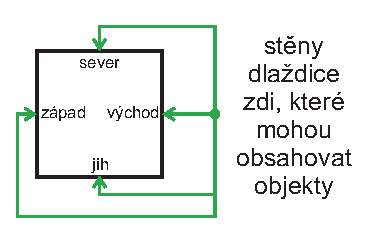
\includegraphics[width=\textwidth]{./img/DM-wall-sides}
        \caption{Dlaždice zeď -- stěny.}
        \label{wall:analyza}
    \end{subfigure}
    \begin{subfigure}[b]{0.45\textwidth}
        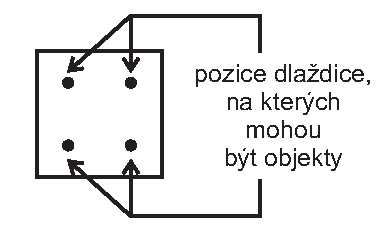
\includegraphics[width=\textwidth]{./img/DM-floor-spaces}
        \caption{Dlaždice podlaha -- pozice.}
        \label{floor:analyza}
    \end{subfigure}
    \caption{Možné pozice pro uložení objektů na dlaždici.}\label{tile-positions:analyza}
\end{figure}

Samotné úrovně jsou pak vždy definovány následujícími seznamy v tomto pořadí:
\begin{itemize}
\item seznam dlaždic -- seřazeny po sloupcích dané úrovně,
\item seznam dekorací příšer,
\item seznam dekorací zdí, 
\item seznam dekorací podlah.
\end{itemize}
Počty jednotlivých dekorací a dlaždic jsou popsány ve vlastnostech úrovní.

\subsection{Textová data}

V binárním souboru jsou často data uložena po slovech procesoru, které v tomto případě mají velikost dvou bajtů. 
V této části souboru jsou uložena data s použitými texty ve hře. Tyto texty používají speciální kódování,
kdy jednotlivé znaky jsou uloženy do slov  (těch procesorových) a každé toto slovo obsahuje tři znaky. Všechny 
texty jsou pak uloženy za sebou v jednom bloku a ke konkrétním textům je přistupováno přes offsety počtu bajtů
od začátku textových dat. Přesný popis je opět k nalezení v komunitní dokumentaci \cite{TechnicalDocumentationFontanel05}.

\subsection{Objekty}

Tyto objekty uložené v souboru \ccc{DUNGEON.DAT} tvoří jednotlivé instance. Odpovídající typy
k těmto instancím jsou potom spolu s jejich neměnnými vlastnostmi uloženy v souboru \ccc{GRAPHICS.DAT},
jehož obsah si rozebereme v následující sekci \ref{dungeon-properties}. Tyto typy se pak ještě dělí do kategorií popsaných dále v této sekci.
Pro určení konkrétního typu má potom každá instance uložen index typu v dané kategorii \cc{instance-type}.
Objekty reprezentující instance obsahují pouze vlastnosti, které jsou rozdílné pro každou konkrétní instanci.

\imgx{instance-type}{Ilustrace vztahu instancí a typů.}

\subsubsection{Identifikátory}

Ke každé instanci objektu existuje unikátní identifikátor, který se skládá z následujících částí:
\begin{itemize}
\item Pozice -- lze buď interpretovat jako světovou stranu, nebo 
	umístění na dlaždici, jedná-li se o podlahu.
\item Kategorie typu objektu -- pro každou kategorii existuje
	v souboru \ccc{DUNGEON.DAT} seznam jejich instancí.
\item Index -- určuje index objektu v seznamu instancí jeho kategorie.
\end{itemize}

Tyto identifikátory se dají chápat jako reference na konkrétní instance objektů \cc{identifier-linklist},
pomocí nichž jsou vytvořeny spojové seznamy. Každá dlaždice pak specifikuje, zda může mít spojový seznam.
Seznam objektových identifikátorů obsahuje první identifikátory spojových seznamů na dlaždicích, které 
je mají. Seznam je uspořádaný pro všechny dlaždice od první do poslední úrovně, vždy po sloupcích odshora dolů \cc{identifier-list}.

\imgx{identifier-linklist}{Ilustrace obsahu identifikátoru a jeho využití ve spojových seznamech.}
\imgx{identifier-list}{Ilustrace uspořádání prvních objektových identifikátorů dlaždic.}

\subsubsection{Předměty}\label{grabable-items}

Předměty jsou objekty, které lze sbírat, používat nebo ukládat k šampionům.
Dělí se do následujících kategorií:
\begin{itemize}
\item \xxx{Zbraně} (weapons) -- lze je vložit šampionům do ruky a ti pak s nimi mohou bojovat.
\item \xxx{Oblečení} (clothes/armor)-- lze jím obléknout šampiony, a tak zvýšit jejich odolnost.
\item \xxx{Svitky} (scrolls) -- obsahují text, který může hráči usnadnit hru.
\item \xxx{Lektvary} (potions) -- dělí se na lektvary modifikující šampionovi schopnosti a na lektvary provádějící nějaké
	akce -- např.: výbuch. Každá instance má vlastnost určující sílu efektu.
\item \xxx{Kontejnery} (containers) -- mohou obsahovat další předměty.
\item \xxx{Různé} (miscellaneous)-- v této kategorii je například jídlo nebo různé předměty, s kterými nelze provádět žádné akce.
\end{itemize}

\subsubsection{Ostatní objekty}
Tyto objekty slouží jako pomocné objekty pro dlaždice a dělí se do následujících kategorií:

\begin{itemize}
\item \xxx{Dveře} (door) -- můžou být pouze na dlaždici typu \xxx{dveře} a obsahují informace, zda-li jsou dveře rozbitelné a jestli 
	mají tlačítko, kterým je lze otevřít.
\item \xxx{Teleport} (teleporter) -- může být pouze na dlaždici typu \xxx{teleport} a definuje cílovou dlaždici a kategorii objektů, které je schopen teleportovat.
\item \xxx{Textové popisky} (texts) -- mohou být pouze na dlaždici typu \xxx{zeď} a obsahují odkaz na konkrétní text do textový dat.
\item \xxx{Skupina nepřátelské entity} (creatures) -- definuje skupinu nepřátelských entity na dlaždici, jejich počet, rozmístění na dlaždici a předměty, které lze získat jejich zabitím.
\item \xxx{Senzory} (sensors/actuators) -- vytvářejí základní mechaniky herních úrovní. Senzory mají daný číselný typ, pomocí kterého hra 
	určí, jakým způsobem je možné senzor
	aktivovat. Po aktivaci senzor buď může provést lokální akci, nebo odeslat zprávu s akcí na vzdálenou 
	dlaždici. Přepínače se pak typicky skládají z několika senzorů. Více o přepínačích a senzorech bude zmíněno
	v sekci \ref{actuator-analyza}. 
\end{itemize}

\section{Data s vlastnostmi objektů -- \ccc{GRAPHICS.DAT}}\label{dungeon-properties}

Soubor \ccc{GRAPHICS.DAT} obsahuje textury dekorací, vlastnosti předmětů a objektů, definici akcí a kouzel.
Formát tohoto souboru nebyl tvůrci uveřejněn, avšak komunitě se opět podařilo data
vyextrahovat. K některým částem také existuje komunitní dokumentace \cite{DMGraphicsDAT}, 
nicméně není ucelená jako v případě dokumentace souboru \ccc{DUNGEON.DAT}. Zároveň 
jsou vyextrahovaná data zveřejněna na webu v HTML formátu (\cite{DMActions}, \cite{DMItems}, \cite{DMItemDescriptors}, \cite{DMSpells}, \cite{DMCreatures}). Z toho důvodů jsme se rozhodli 
pro využití již extrahovaných dat v HTML formátu. Dále následuje podrobnější popis využitého obsahu souboru.

\subsection{Akce a komba}\label{action-combos}

S předměty je možné provádět akce. Množina akcí pro daný předmět se nazývá kombo a obsahuje 
až tři akce. Ve hře je k dispozici 44 akcí a stejný počet komb. Kompletní seznam jednotlivých
akcí a komb lze nalézt v komunitní dokumentaci \cite{DMActions}. Zde si popišme alespoň jejich vlastnosti.

\medskip

Vlastnosti akcí jsou:
\begin{itemize}
\item \xxx{název} (name) -- textový popis akce ve hře,
\item \xxx{zkušenosti} (experience gain) -- počet zkušeností získaných po provedení akce,
\item \xxx{dovednost} (skill) -- identifikátor dovednosti, která získá zkušenosti,
\item \xxx{obrana} (defense modifier) -- modifikátor obrany při používání akce,
\item \xxx{výdrž} (stamina) -- modifikátor výdrže nutné pro provedení akce, 
\item \xxx{pravděpodobnost provedení akce} (hit probability),
\item \xxx{zranění} (damage) -- modifikátor pro výpočet konečného zranění nepřítele, 
\item \xxx{únava} (fatigue) -- doba, po kterou nelze provádět žádné akce. 
\end{itemize}

\medskip

Vlastnosti pro každou akci komba jsou:
\begin{itemize}
\item index akce ze seznamu akcí (action index), 
\item úroveň dovednosti (skill level) -- minimální úroveň dovednosti pro úspěšné provedení akce. 
\end{itemize}


\subsection{Předměty}\label{item-descriptors}

Ke každému typu předmětu existují v tomto souboru popisovače vlastností \cite{DMItemDescriptors}.
Pro každý předmět jsou definovány následující vlastnosti:  
\begin{itemize}
\item \xxx{globální identifikátor} (global item index) -- unikátní identifikátor, který je použit k identifikaci konkrétního typu předmětu například v přepínačích,
\item \xxx{index útočného komba} (attack combo),
\item \xxx{lokace} (carry location) -- místo, na kterou část těla, nebo do kterého inventáře šampiona lze předmět vložit,
\item \xxx{index v kategorii} (index in its category) -- index typu předmětu v dané kategorii.
\end{itemize}

Globální identifikátor lze z instance předmětu získat pomocí jeho kategorie a indexu typu předmětu,
který má každá instance předmětu. Každý předmět má také definovanou hmotnost. Zbraně a oblečení mají navíc
definované následující vlastnosti, jejichž hodnoty lze nalézt v komunitní dokumentaci \cite{DMItems}.

\medskip

Zbraně:
\begin{itemize}
\item \xxx{poškození} (damage) -- hodnota zranění aplikovaná při útoku na nepřítele,
\item \xxx{kinetická energie} (energy) -- hodnota udává, jak daleko lze zbraň hodit,
\item \xxx{střelné poškození} (shoot damage) -- hodnota dodatečného poškození u střelných zbraní.
\end{itemize}

Oblečení:
\begin{itemize}
\item \xxx{síla brnění} (armor strength) -- obrana, kterou oblečení poskytuje, 
\item \xxx{odolnost proti útokům ostrými předměty} (sharp resistance). 
\end{itemize}

\subsection{Kouzla a symboly}\label{magic-symbols}

Další častí dat uložené v souboru \ccc{GRAPHICS.DAT} jsou vlastnosti kouzel. Pojď\-me si nejprve přiblížit,
jak se ve hře kouzla přesně vyvolávají. Každé kouzlo je složeno z několika symbolů, přičemž první 
z nich je speciální a jde o tzv. ,,power symbol". Power symbol určuje, jak bude celkové kouzlo silné.
Další symboly už určují konkrétní kouzlo. Každé vyvolání symbolu stojí šampiona \xxx{manu}. Po stanovení 
všech symbolů může šampion vyvolat samotné kouzlo. Vyvolání kouzla může selhat, pokud nemá šampion 
dostatečnou úroveň dovednosti vyžadované kouzlem. Datový soubor tedy obsahuje pro každý symbol při odpovídajícím
power symbolu množství potřebné many pro jeho vyvolání. Dále obsahuje následující vlastnosti kouzel \cite{DMSpells}:

\begin{itemize}
\item \xxx{Obtížnost} (Difficulty) -- modifikátor obtížnosti vyvolání kouzla,
\item \xxx{Doba trvání} (Duration) -- po tuto dobu nemůže šampion vyvolávat další kouzla,
\item \xxx{Úroveň dovednosti} (Skill level) -- postačující úroveň určité dovednosti pro úspěšné vyvolání kouzla.
\end{itemize}

\subsection{Nepřátelské entity}\label{properties-creatures}

Poslední částí obsaženou v souboru \ccc{GRAPHICS.DAT}, kterou jsme využili, jsou vlastnosti nepřátelských entit.
Následující výčet obsahuje vlastnosti, které implementuje nový engine. 
\begin{itemize}
\item \xxx{Doba pohybu} (Movement duration) -- doba, po které se entita rozhodne změnit pozici.
\item \xxx{Doba útoku} (Attack duration) -- doba, po které může entita provést útok.
\item \xxx{Síla brnění} (Armor) -- určuje odolnost proti útokům.
\item \xxx{Zdraví} (Base health) -- hodnota použitá pro výpočet zdraví nových nepřátelských entit.
\item \xxx{Síla útoku} (Attack power) -- hodnota pro výpočet útoku.
\item \xxx{Otrava} (Poison)  -- určuje, jak velkou otravu způsobí útok. 
\item \xxx{Obrana} (Defense) -- určuje obtížnost pro šampiona, se kterou je entita zraněna. 
\item \xxx{Detekce} (Detection range) -- určuje vzdálenost, na kterou detekuje nepřítele. 
\item \xxx{Odolnost proti ohni} (Fire resistance) -- odolnost proti kouzlům způsobující ohnivý útok.
\item \xxx{Odolnost proti jedu} (Poison resistance) -- odolnost proti kouzlům způsobující jedový útok.
\item \xxx{Pravděpodobnosti zranění částí těla} (Wounds) -- pravděpodobnost pro každou část těla nepřítele, s kterou ji entita zraní.
\end{itemize}

Celý seznam vlastností je možné nalézt v komunitní dokumentaci \cite{DMCreatures}.


\section{Parsování vstupních dat}\label{level-parsing}

V době implementace této části práce nebylo jasné, zda nalezená dokumentace \cite{TechnicalDocumentationFontanel05} bude dostatečná
pro splnění práce. Parser je proto oddělen od zbytku enginu do zvláštní assembly, která nereferencuje žádnou knihovnu
pro zobrazování grafiky. Cílem této assembly je tedy pouze převést struktury obsažené ve vstupních datech do odpovídajících
datových tříd v jazyce C\#. Tento balík dat se potom předá enginu, který z něj nich vytvoří herní úrovně. Toto schéma 
znázorňuje následující obrázek \ref{parser-preview}.

\imgx{parser-preview}{Ilustrace vztahu parseru vůči enginu.}

\subsection{Herní úrovně -- \ccc{DUNGEON.DAT}}\label{dungeon-parser}

Parsování herních úrovní je rozděleno do dvou fází. V první fázi probíhá transformace dat objektů \vref{dungeon-objects} ze souboru \ccc{DUNGEON.DAT}
 na odpovídající objekty v jazyce C\#. V druhé fázi jsou pak objekty z první fáze upraveny,
aby měly přehlednější strukturu. 


\subsubsection{První fáze}

V této fázi je nejprve vytvořen datový objekt, který bude shromažďovat všechny ostatní data. Tento objekt obsahuje:

\begin{itemize}
\item metadata z hlavičky souboru -- to jsou zejména velikosti všech seznamů s objekty \vref{dungeon-objects} a počet map,
\item seznamy objektů -- to jsou seznamy objektů jazyka C\# vzniklé rozparsováním odpovídajících dat objektů v souboru,
\item seznam herních úrovní -- to jsou objekty reprezentující data herních úrovní, které obsahují jejich vlastnosti \vref{dungeon-objects}
 a seznam jejich dlaždic, dekorací, atd. 
\end{itemize}

Dále parser rozparsuje všechna data vstupního souboru dle komunitní dokumentace \cite{TechnicalDocumentationFontanel05} a vytvoří z nich 
adekvátní objekty, které uloží do zmíněného datového objektu. Ilustrace této fáze je na obrázku \ref{DM-parser}.

\subsubsection{Druhá fáze}
Po skončení první fáze je struktura vzniklého datového objektu podobná struktuře souboru \ccc{DUNGEON.DAT}. Tím máme namysli, že
například spojové seznamy jsou reprezentovány pomocí objektových identifikátorů \vref{dungeon-objects}, což není příliš intuitivní a pro práci 
s těmito daty by engine musel rozumět jejich formátu. Navíc spojové seznamy obsahují objekty různých typů. Proto pro zjednodušení práce enginu
s těmito daty jsou v datových objektech inicializovány ještě následující položky: 
\begin{itemize} 
\item seznam sbíratelných předmětů,
\item seznam senzorů,
\item seznam popisků,
\item seznam nepřátelských entit,
\item položka dveří pro dlaždici typu dveře,
\item položka teleport pro dlaždici typu teleport,
\item a pro dlaždici typu zeď a podlaha stanoví identifikátory náhodných dekorací.
\end{itemize} 

Na počátku vývoje projekt neobsahoval druhou fázi, její vytvoření vedlo k zjednodušení kódu v enginu.

\subsection{Vlastnosti objektů -- \ccc{GRAPHICS.DAT}}

Pro sestavení herních úrovní potřebuje engine také vlastnosti společné pro všechny konkrétní typy objektů ze
souboru \ccc{DUNGEON.DAT}. Jak bylo zmíněno v sekci \ref{dungeon-properties}, tyto vlastnosti jsou v originální hře v souboru \ccc{GRAPHICS.DAT}.
Nicméně tato data již existují vyextrahovaná v HTML formátu, a proto jsme je použili namísto původních dat.
Ke zjednodušení parsování dat z HTML souborů byla
použita knihovna HTML Agility Pack \cite{HtmlAgilityPack}. Pro každé typy vlastností jsou pak vytvořeny odpovídající datové objekty,
které jsou uloženy do seznamů ve výsledném datovém objektu zmíněného v předchozí
sekci \ref{dungeon-parser}. V této části jsou získána data vlastností všech objektů \vref{dungeon-objects} až na kouzla.
Vlastnosti kouzel jsou rozparsovány v enginu přímo do objektů v něm použitých. Proto by případné vytváření datových souborů
v této vrstvě bylo zbytečné. Celý proces zobrazuje diagram na obrázku \ref{DM-parser}.

\imgx{DM-parser}{Průběh parsování herních dat.}

\section{Výběr frameworku pro práci s grafickým výstupem}

Po úspěšném rozparsování herní dat se bylo třeba rozhodnout, kterou knihovnou použít pro zobrazení grafického výstupu enginu. 
Aby se bylo možné soustředit hlavně na samotný návrh enginu \aref{aim-extensibility}, použili jsme framework, se kterým už jsme měli nějaké zkušenosti.
Jedná se o XNA Framework od firmy Microsoft. Nicméně tento framework již není firmou nadále podporován a vyvíjen, proto jsme nakonec využili 
klon MonoGame \cite{MonoGame}. Výhodou této volby je také to, že framework je multiplatformní. Jeho tvůrci tvrdí, že podporuje platformy
iOS, Android, MacOS, Linux, Windows, OUYA, PS4, PSVita, Xbox One.

\section{Reprezentace jádra enginu}\label{a:engine-core-section}

O samotnou herní smyčku se stará framework MonoGame, který na jádru enginu volá aktualizační a vykreslovací obsluhy.
Jádro enginu obsahuje následující tři důležité komponenty:
\begin{itemize}
\item Hráč -- tato komponenta zajišťuje interakci s uživatelem. Skrze ni lze ovládat hráčovu skupinu šampionů, sbírat předměty nebo bojovat.
\item Builder herních úrovní -- tato komponenta zajišťuje sestavování herních úrovní.
\item Objekt obsahující factories -- pro každý typ popsaný v sekci \ref{dungeon-properties} existuje odpovídající
	factory obsahující jeho vlastnosti. Factories mohou vytvářet objekty, jejichž typ reprezentují. Toto bude konkrétně
	specifikováno později \vref{item-factories}, nicméně důležité je, že skrze jádro enginu lze k těmto factories přistupovat.
\end{itemize}
Podrobnosti o jádře enginu jsou ve vývojové dokumentaci \vref{a:engine-core-section}.

\section{Reprezentace dlaždic}\label{tile-representation}

V originální hře jsou dlaždice vždy uloženy v obdélníkovém poli (viz sekce \ref{dungeon-objects} a obr \ref{tile-representation-img} vlevo).
To znamená, že dlaždice, které nejsou využity pro~chodby, jsou vždy vyplněny zdmi. Jelikož jedním z cílů této práce je udělat engine co 
nejrozšiřitelnější \aref{aim-extensibility}, rozhodli jsme se tento problém vyřešit o něco obecněji (viz obr. \ref{tile-representation-img} vpravo).
Každá dlaždice je vrchol grafu, a pokud 
jsou dvě dlaždice sousední, jsou mezi nimi hrany oběma směry, to dohromady tvoří obousměrně orientovaný graf.
Nicméně, pro dlaždice stále platí, že mají nanejvýš čtyři sousedy a jsou uspořádané do mřížky. Tato reprezentace pro hodně řídké mapy může ušetřit paměť.
Avšak důležitější je, že při takové reprezentaci lze jednoduše získat sousedy pouze ze znalosti konkrétní dlaždice. V této 
podobě by bylo navíc jednoduší engine upravit tak, aby dlaždice nemusely být na mřížce a aby mohly mít více sousedů.

\imgx{tile-representation-img}{Uložení dlaždic v originálním vs. tomto enginu.}

Předchozí rozhodnutí také vede k tomu, že již nejsou potřeba dlaždice typu zeď \cc{tile-representation-img}, jelikož její stěny mohou být definovány ve 
dlaždicích typu podlaha \cc{tileside-move}. Při vytváření podlahy je pak nutné číst i její sousední dlaždice. Pokud je soused daným směrem zeď, 
vytvoří se na této straně stěna a soused není nastaven. V opačném případě je soused nastaven na odpovídající dlaždici.
Zprávy původně cílené zdím je také třeba posílat na odpovídající dlaždice podlahy \cc{tile-representation-img}. Tato reprezentace zdí opět vede k
vyšší flexibilitě, jelikož případné místo využité původními dlaždicemi typu zdi lze využít jiným způsobem.

\imgx{tileside-move}{Ilustrace přesunu stěn do dlaždice \xxx{podlahy}}

Pokud jsou tedy stěny součástí dlaždic, je třeba vyřešit jejich reprezentaci. Buď je možné, aby veškeré funkce stěn obsahovala přímo
dlaždice, a nebo je možné tyto části delegovat do zvláštních objektů. Ze začátku byl v enginu použit první zmiňovaný způsob. Nicméně 
tato reprezentace není příliš vhodná, protože potom samotná dlaždice řeší funkce, které k ní přímo nenáleží.
Nakonec tato reprezentace byla změněna a v enginu byla použita druhá zmiňovaná možnost. Vedlo k ní zejména oddělení zobrazovací vrstvy 
od logické. Výhoda tohoto přístupu byla kromě samotného oddělení kódu i možnost znovu použití kódu za pomocí dědičnosti. 
Například třída reprezentující stěnu, která obsahuje přepínač, může dědit ze třídy reprezentující prázdné stěny. 
Avšak ukázala se i nevýhoda tohoto přístupu, a to, že komunikace směrem ze stěny k dlaždici je trochu těžkopádná.
Buď by bylo zapotřebí předat zdi referenci na jejich rodičovské dlaždice, nebo by se musely
použít události. Pokud to bylo v některých případech nutné, přiklonili jsme se k použití událostí.

\section{Přepínače}\label{actuator-analyza}
Přepínače tvoří základní mechaniky v herních úrovních Dungeon Masteru, mohou být buď na stěnách, nebo na podlaze. 
Na stěnách je lze aktivovat kliknutím myši a na podlaze potom přesunutím hráče na dlaždici s přepínačem. Aktivace ještě
může být podmíněna dalšími faktory: obsah daného typu předmětu v ruce nebo směr, kterým je hráč otočen.  

Ve skutečnosti se každý přepínač skládá z řady senzorů a platí, že:
\begin{itemize}
\item poslední senzor určuje dekoraci přepínače,
\item při pokusu o aktivaci přepínače dojde postupně k pokusu aktivace každého senzoru,
\item každý senzor může definovat akci, kterou provede, pokud byl aktivován.
\end{itemize}

Senzor má následující vlastnost:
\begin{itemize}
\item Typ (type) -- číselné označení, dle kterého originální herní engine určí způsob aktivace.
\item Akce (action type) -- může být buď lokální, nebo vzdálená. Pro lokální akce je to zarotování sekvencí senzorů 
	přepínače nebo přidání zkušeností hráči. Pro vzdálené akce je to odeslání zprávy \vref{dungeon-objects} na danou cílovou dlaždici. 
\item Data (data) -- pro každý typ senzoru se může obsah lišit.  
\item Zpoždění (action delay) -- doba, po které se provede akce. Jedna jednotka tohoto času je rovna 1/6 sekundy.
\item Opačný efekt (revert effect) -- liší se dle typu senzoru, nicméně většinou otáčí podmínku aktivace pro daný typ senzoru. 
\item Opakovatelnost (once only) -- určuje, zda lze senzor aktivovat neomezeně či pouze jednou.
\item Dekorace (decoration) -- číselný identifikátor dekorace, jehož hodnota mínus jedna slouží jako index 
do právě používaných dekorací, které jsou definovány pro každou herní úroveň. Dekorace s číslem nula 
potom označuje, že nemá být použita žádná dekorace. 

\end{itemize}

Výše popsaný systém přepínačů přináší hned několik problémů:
\begin{enumerate}[label=\textbf{P\arabic*}]
\item\label{actuator-unclear} Z technické dokumentace \cite{TechnicalDocumentationFontanel05} není vždy jasně zřejmé, jaká je aktivační podmínka senzoru pro určitý typ.
\item\label{actuator-effective} Jakým způsobem efektivně a přehledně rozparsovat data senzorů, když mají tolik nezávislých vlastností.
\item\label{actuator-representation} Jak reprezentovat přepínače v novém enginu.
\item\label{actuator-remote-actions} Jakým způsobem provádět vzdálené akce.
\end{enumerate}

\subsection{Příklady}
Pro ujasnění celého konceptu přepínačů si pojďme ukázat několik příkladů. Textový popis aktivační podmínky senzorů pro jednotlivé 
jejich typy může být nalezen v komunitní dokumentaci \cite{TechnicalDocumentationFontanel05}. Přesná funkce senzorů pak může být nalezna
v dekompilovaných zdrojových kódech \cite{DMDecompilation} v následujících funkcích, které jsou v souboru \ccc{SENSOR.C}:

\begin{itemize}
\item \ccc{F275\_aszz\_SENSOR\_IsTriggeredByClickOnWall} -- chování pro senzory na zdech,
\item \ccc{F276\_qzzz\_SENSOR\_ProcessThingAdditionOrRemoval} -- chování pro senzory na podlaze.
\end{itemize}

\subsubsection{Držák na pochodně}

Držák na pochodně \cc{torch-actuator} se skládá ze dvou senzorů, jehož data a umístění je znázorněno na obrázku \ref{torch-actuator}. Dlaždice
na pozici (0, 0) je typu \xxx{podlaha}, takže na ní může být hráč a může kliknout na přepínač na stěně dlaždici \xxx{zdi} na pozici (1, 0).

Senzor na první pozici je typu~0, což znamená, že tento senzor nelze aktivovat. Senzor může pouze zobrazovat svoji dekoraci, pokud je na posledním 
místě sekvence, ostatní jeho vlastnosti nejsou využity. Dekorace má hodnotu 7, což znamená, že bude použita dekorace stěn pro danou herní úroveň
s indexem 6, která v tomto příkladu reprezentuje dekoraci prázdného držáku na pochodně.

Senzor na druhé pozici je typu~13, což znamená, že tento senzor lze aktivovat buď pokud má hráč prázdnou ruku a ve zdi je uložen předmět, jehož
globální identifikátor je roven položce data, nebo pokud má hráč v ruce předmět s globálním identifikátorem předmětu rovným položce data a zeď neobsahuje
žádný předmět. Položka data s číslem 4 reprezentuje globální identifikátor předmětu pochodně. Položku akce tento senzor nevyužívá. Dekorace s číslem
8 potom reprezentuje plný držák na pochodně. Zpoždění má v tomto případě hodnotu 1, což znamená, že se akce provede 1/6 sekundy po aktivaci senzoru.
Akce senzoru je lokální, což znamená, že po aktivaci senzoru může být provedena rotace senzorů v sekvenci přepínače nebo přidání zkušenosti hráči. 
V tomto případě se provádí rotace senzorů. Veškeré akce přepínače v tomto příkladě dělá tento druhý senzor.

Při aktivaci přepínače se tedy vezme pochodeň uložená ve zdi a vloží se hráči do ruky. Následně se provede rotace senzorů, čímž se zobrazí
dekorace prázdného držáku na pochodně. Při opětovné aktivaci přepínače se vloží pochodeň z ruky hráče zpět do zdi. A následuje opět rotace senzorů, čímž
se zobrazí opět dekorace plného držáku na pochodně.

\imgx{torch-actuator}{Ilustrace přepínače pro držák pochodní.}

\subsubsection{Páka}

Páku tvoří dva senzory stejného typu~1, jejichž data a umístění je znázorněno na obrázku \ref{lever-actuator}. 
Dlaždice na pozici (0, 0) je typu \xxx{podlaha}, takže na ní může hráč vstoupit a kliknout na přepínač na stěně dlaždice \xxx{zdi} na pozici (0, 1).
Na pozici (1, 0) je potom otevřená dlaždice typu \xxx{jáma}, na kterou nelze vstoupit, aniž by do ní hráč spadl.  
Senzor typu 1 lze potom aktivovat nezávisle na tom co má hráč v ruce. Položku data tento senzor nepoužívá. 

První senzor má dekoraci číslo 8, která v tomto příkladě reprezentuje páku nahoru. Zpoždění má hodnotu 1, což znamená, že se akce senzoru provede
po 1/6 sekundy. Akce je pro tento senzor lokální, což znamená, že se nevyužije položka akce, ale provede se rotace senzorů, jelikož je nastavena 
položka rotace. 

Druhý senzor má dekoraci 9, která reprezentuje v tomto příkladě dekoraci s pákou nahoře. Akce je nastavena na nelokální, takže se provede vzdálená
akce, jejíž pozici určuje položka pozice tj. (1, 0). Položka akce pak reprezentuje přehození stavu, které se provede opět 1/6 sekundy od aktivaci. 

Po aktivaci přepínače tedy nejprve dojde k rotaci senzorů způsobené prvním senzorem -- takže se zobrazí dekorace páky dole.
Se zpožděním 1/6 sekundy pak druhý senzor odešle \xxx{jámě} na pozici (1, 0) zprávu, aby přehodila její stav -- což znamená, že se jáma zavře.
Opětovná aktivace přepínače provede opět rotaci senzorů, takže se zobrazí znovu dekorace páky nahoře. Druhý senzor následně odešle \xxx{jámě} zprávu 
o změně stavu, takže se \xxx{jáma} opět otevře.

\imgx{lever-actuator}{Ilustrace přepínače reprezentující páku.}


\subsubsection{Tlačítko}

Toto tlačítko se skládá opět ze dvou senzorů typu~1 a rozmístění je analogické jako v předchozím příkladu \cc{button-actuator}.
Oba senzory potom mají vzdálenou akci na dlaždici (1, 0) -- první senzor vyšle deaktivační zprávu a druhý aktivační \cc{button-actuator}.
První senzor nemá nastavenou dekoraci a druhý senzor má dekoraci s číslem 1, která reprezentuje tlačítko. Akce prvního senzoru
se provede se zpožděním jedné sekundy a akce druhého se zpožděním šesti sekund. 

Po aktivaci přepínače je tedy skrze první senzor odeslána deaktivační zpráva na dlaždici typu \xxx{jáma} se zpožděním jedné sekundy.
Po obdržení této zprávy se jáma zavře a hráč na ni tak může vstoupit.  Druhý senzor poté po šesti sekundách provede 
aktivaci dlaždice typu \xxx{jáma}, která povede na její opětovné otevření.

\imgx{button-actuator}{Ilustrace přepínače reprezentující dočasné tlačítko.}


\subsection{Reprezentace přepínačů}
První tři body problémů  (viz \ref{actuator-unclear}, \ref{actuator-effective}, \ref{actuator-representation}) řeší tato sekce.

\subsubsection{První reprezentace}\label{rep-v1}

Jako první způsob jsme se rozhodli vždy pro několik sekvencí senzorů vytvořit objekt, který měl stejné nebo o něco obecnější vlastnosti než dané sekvence.
Z počátku se totiž zdálo, že jen výjimečně jsou sekvence senzorů větší či složitější. Proto jsme se rozhodli vytvořit v
novém enginu objekty, které mají obecnější vlastnosti, a tak mohou být použité pro několik podobných sekvencí. Dle určité sekvence senzorů se poté
objektu inicializují jeho vlastnosti. Celou situaci ilustruje obr. \ref{actuator-object}.

\imgx{actuator-object}{Ilustrace transformace sekvence senzorů na objekt přepínač.}


Konkrétním příkladem může být objekt přepínače reprezentující držák na pochodně \cc{actuator-object-example}.
Kdy první sekvence reprezentuje držák s pochodní a druhá držák bez ní -- při vytváření objektu držáku se pak specifikuje, zda má či nemá pochodeň. 

\imgx{actuator-object-example}{Ilustrace transformace sekvence senzorů na objekt přepínač.}

Tento způsob sice řeší problém samotné reprezentace \vbref{actuator-representation}, ale později se ukázalo, že velice nevhodně. Například
kód převádějící sekvence na přepínače je složitý a nepřehledný. Bylo také složité vytvořit přepínač podle technické dokumentace \cite{TechnicalDocumentationFontanel05}
tak, aby fungoval správně. Popis v dokumentaci \cite{TechnicalDocumentationFontanel05} také není dostatečně přesný pro vytvoření tohoto úkolu.
I proto čím více přepínačů jsme tímto způsobem naimplmentovali, tím více se ukazovalo problémů. Nakonec jsme dospěli k závěru, že tento způsob reprezentace je nemožný.

\subsubsection{Druhá reprezentace}

Tato reprezentace se snažila vyřešit problém nepřehlednosti kódu\vbref{actuator-effective} převádějícího sekvence na objekty přepínačů.
Proto je i zde použit typ objektu přepínač z první reprezentace v sekci \ref{rep-v1}. Parsování sekvence senzorů jsme se rozhodli udělat pomocí konečného 
automatu. Tedy tak, že pro každý objekt přepínače existovaly předdefinované sekvence senzorů. Konečný automat potom pomocí vstupní sekvence
identifikoval výsledný objekt přepínače. Při inicializaci objektu přepínače zde pak byla sekvence jasně definovaná, což řešilo problém s přehledností \vbref{actuator-effective}.
Později se však ukázalo, že i malá změna v sekvenci senzorů může generovat podobný objekt. Takže by bylo třeba
spoustu předdefinovaných šablon, které by se lišily ve drobnostech. Tím se ukázalo, že tento přístup není dostatečně obecný a nelze jej tedy použít. 

\subsubsection{Třetí reprezentace -- výsledná}

Tato reprezentace se oproti předchozím snažila přiblížit co nejvíce k systému použitém v enginu originální hry.
K dosažení tohoto cíle jsme se rozhodli použít dekompilované zdrojové kódy \cite{DMDecompilation} hry. Tím
je vyřešen problém nedostatečné dokumentace ve věci přepínačů\vbref{actuator-unclear}.

Vytvořili jsme tedy objekt přepínač, který má v sobě sekvenci senzorů tak, jako tomu je v originální hře.
Tím je vyřešen i problém nepřehlednosti převodního kódu\vbref{actuator-effective}, jelikož jsou tyto reprezentace téměř identické.
S využitím zdrojových kódů jsme vytvořili odpovídající objektově orientovaný kód v jazyce C\#. Tato reprezentace
tak zajišťuje maximální korektnost implementace a přitom poskytuje možnost rozšíření -- což je jedním z cílů této práce  (viz bod \ref{aim-extensibility}). 
Je tedy možné vytvořit nové senzory, které budou mít vlastní aktivační podmínky a ty následně použít v přepínačích.
V originálním enginu je toto rozšiřovaní značně omezené, jednotlivé typy senzorů se tam odlišují jednobajtovým číselným identifikátorem.
Ale jelikož jsme nechtěli rozšiřování enginu limitovat pouze na tento způsob vytváření senzorů, je možné si vytvořit přepínač, který
bude fungovat na úplně jiné bázi. Takže případné nové přepínače nemusí vůbec senzory používat. 

\subsection{Reprezentace zprávy přepínače}\label{actuator-message-representation}

Jak již bylo řečeno \vref{dungeon-objects}, celý systém mechanik herních úrovní je závislý na posílání zpráv. 
V originální hře je cíl odeslané zprávy vázán na její souřadnice dlaždice. 
Jelikož jsme se v enginu nechtěli vázat na tyto pevné souřadnice, rozhodli jsem se namísto nich
cílovou dlaždici identifikovat její referencí. To by případně ulehčilo práci při transformaci enginu tak, aby
dlaždice mohly mít více sousedů nebo aby nemusely být na pevné mřížce \vref{tile-representation}.
Při takovéto reprezentaci však nastává problém s inicializací dlaždic a přepínačů \vref{level-inicialization}.

V originální hře lze mezi dlaždicemi posílat pouze jeden typ zprávy. Jelikož cílem této práce je udělat engine
co nejrozšiřitelnější  (viz bod \ref{aim-extensibility}), engine poskytuje za určitých podmínek používat i jiné typy zpráv.
Těmito podmínkami jsou:
\begin{itemize}
\item Vlastní zprávy lze zasílat pouze vlastně vytvořeným dlaždicím, které na daný typ zprávy musí být připraveny.
\item Všechny dlaždice musí umět přijímat originální typ zprávy -- nicméně nemusí na ně reagovat.
\item Třída reprezentující vlastní zprávu musí být potomkem originální zprávy v hiearchii dědičnosti jazyka C\#.
\end{itemize}

\section{Reprezentace entit}

V originální hře existují pouze dva typy živých objektů, tj. nepřátelské entity a šampioni. Za účelem udělat engine
co nejrozšiřitelnější \aref{aim-extensibility} jsme se rozhodli rozdělit entity na živé a neživé.   
Entitou je v tomto enginu každý objekt, s jehož vlastnostmi může interagovat nějaká akce \vref{action-combos}.
Například akce útok může entitu zranit nebo poškodit  (pokud je neživá). Příkladem použité neživé entity 
jsou dveře, které je možné rozbít útokem. Živé entity disponují následujícími atributy:

\begin{itemize}
\item vlastnosti -- jsou to vlastnosti jako zdraví, odolnost,  atd.  (viz sekce \ref{properties-skills}),
\item dovednosti -- to ve výsledku znamená, že jsou schopny používat akce,
\item relaci vůči ostatním živým entitám -- určuje, zda jsou vůči daným entitám přátelské či nepřátelské,
\item části těla a inventáře,
\item poloha na dlaždici -- definuje, jaké části dlaždic mohou zaujímat.
\end{itemize}

Každý z těchto bodů lze rozšířit, což může být užitečné v případě použití enginu pro implementaci jiné hry než Dungeon Master. 

\subsection{Vlastnosti}\label{entity-properties}

V původní hře jsou vlastnosti šampionů \vref{properties-skills} a nepřátelských entit \vref{properties-creatures} pevně definované. 
Několik vlastností nepřátelských entit je odlišných od tě šampionových, nicméně ve většině se shodují.
S těmito odlišnostmi musí počítat akce, které modifikují vlastnosti entit. Pokud entita nějakou vlastností nedisponuje, je vrácena 
vlastnost se základní hodnotou. Například pokud provádíme akci útok magickou ohnivou koulí a entita nemá žádnou z vlastností
odolnost proti magii či odolnost proti ohni, výsledný útok akce nebude nijak modifikován. 

 \subsection{Dovednosti}

V originální hře mají šampioni pevně definované dovednosti \vref{properties-skills}, jako je tomu v případě vlastností.
I v tomto bodě se nový engine snaží o větší dynamičnost. Opět platí, že každá entita nemusí mít všechny dovednosti.
Pokud je po entitě vyžadována dovednost, kterou entita nedisponuje, je její úroveň nulová.
V originální hře jsou dva typy dovedností: základní a skryté. Pokud některá akce vylepšuje skrytou dovednost,
rozdělí se získané zkušenosti mezi obě dovednosti \vref{properties-skills}. Tento koncept schopností není v enginu vyžadován a 
záleží potom na konkrétní implementaci dovednosti. Ta také specifikuje množství zkušeností nutné pro 
získání nových úrovní. Implementace dovedností pro hru Dungeon Master odpovídá té ve zdrojových kódech hry \cite{DMDecompilation},
konkrétně v následujících funkcích  v souboru \ccc{CHAMPION.C}:

\begin{itemize}
\item \ccc{F304\_apzz\_CHAMPION\_AddSkillExperience} -- přidání zkušeností dané dovednosti.
\item \ccc{F303\_AA09\_CHAMPION\_GetSkillLevel} -- získání úrovně dané dovednosti.
\end{itemize}

\subsection{Relace mezi entitami}
Další funkcí, kterou oproti originálu engine umožňuje, je definovat pro entity jejich nepřátele. Každá živá entita má token identifikující
skupinu. Entity v této skupině jsou mezi sebou přátelské. Každá entita si může nadefinovat svoje nepřátelské tokeny.
Podle vzoru originálu jsou v hře pouze dva relační tokeny -- první pro šampiony a druhý pro nepřátelské entity. Nicméně
celý tento systém je navržen právě pro stanovení obecnějších vztahů mezi entitami a to může být aplikováno v libovolném rozšíření hry.
 
\subsection{Tělo a inventáře}
Každá živá entita má definované části těla. Oproti originálu, kde se řeší pouze části těla šampionů,
zde je možné definovat tělo pro každou entitu. Je tak možné pracovat s částmi těla entit, které nemají humanoidní formu.
Některé části těla se dají použít jako úložiště předmětů, ty potom mají nadefinováno s jakým typem úložiště jsou kompatibilní.
Tato reprezentace principiálně umožňuje podporu následujícího příkladu. Pokud máme lidské a medvědí nohy, tak lidské
kalhoty by měly jít nasadit pouze na lidské nohy, nikoliv na medvědí. Naopak medvědí chrániče na nohy půjdou nasadit pouze na
nohy medvědí. Takto pokročilejší mechanismy v originální hře nejsou použity, předměty tam mohou sbírat pouze šampioni. Nicméně
tyto mechanismy jsou k dispozici při použití tohoto enginu k implementaci jiné hry.

Předměty lze pak dále ukládat do dalších externích úložných prostorů. 
Mezi taktové úložiště patří například batoh, kapsa, truhla, toulec atd.
O velikosti a typu těchto úložišť opět rozhoduje tvůrce konkretních 
entit. Avšak stejně jako v originální hře, i tato instance má implementované 
úložiště pouze pro šampiony.

\section{Reprezentace předmětů}\label{item-factories}

V herních úrovních jsou různě rozmístěné předměty, které lze sbírat a ukládat si je do inventářů šampionů.
Každý takový předmět náleží do nějaké kategorie (zbraň, lektvar, atd. -- viz sekce \ref{grabable-items}). Všechny 
tyto kategorie obsahují několik typů předmětů. Pro každý typ předmětu pak existuje jednoznačný globální identifikátor \vref{item-descriptors}.
Identifikátory jsou použité například v přepínačích pro identifikaci typu předmětu, dle kterého se pak rozhodnou, 
zda se mají aktivovat či nikoliv. Platí tedy, že všechny instance daného typu předmětu mají stejný identifikátor.

Z počátku jsme pro stanovení identifikátorů zvolili stejnou strategii jako tvůrci originální hry, tedy každá
instance měla daný číselný identifikátor.
Nicméně takto zvolený způsob reprezentace identifikátorů by byl nepřehledný pro případné rozšiřitele, jelikož
by nemuselo být jasné, které identifikátory už jsou obsazené a které nikoliv. Dále v počátcích každá instance
předmětu měla všechny jeho vlastnosti a to i ty, které byly společné pro všechny instance daného typu \vref{item-descriptors}.

Pro splnění cíle \ref{aim-extensibility} této práce bylo zapotřebí reprezentaci předmětů vylepšit.
Řešením problému bylo delegování společných vlastností předmětů do zvláštních tříd \cc{item-factories}, které odpovídají jednotlivým identifikátorům.
Tyto třídy navíc slouží jako factories na předměty daného typu. Reference na konkrétní instanci třídy pak slouží jako identifikátor.
To ale znamená, že reference na tyto factories jsou potřeba pro vytváření přepínačů. Z toho důvodu je součástí jádra enginu
objekt obsahující všechny factories splňující tento vzor \vref{a:engine-core-section}.

\imgx{item-factories}{Ilustrace vztahu objektů a jejich factories.}

Každá factory na předměty má také následující atributy:
\begin{itemize}
\item hmotnost, 
\item jméno, 
\item kombo -- definuje akce, které lze s předměty provádět,  
\item definice míst v inventáři, kam lze předmět uložit. 
\end{itemize}

\section{Reprezentace komb a akcí}

Každý typ akce definuje svoji factory, která je uložena v jádře enginu \vref{a:engine-core-section} -- jako je tomu v případě předmětů.
Tyto factories obsahují vlastnosti o akci \vref{action-combos}, které také určují požadavky pro provedení dané akce.
Pomocí factory lze pak vytvořit samotný objekt reprezentující konkrétní akci, kterou lze následně vyvolat určitým 
směrem (sever, východ, jih, západ). Jak podmínky vytvoření akce, tak její provedení je naimplementováno dle dekompilovaných
zdrojových kódů \cite{DMDecompilation} originální hry. Každá factory na předměty má potom specifikovaný seznam typů akcí,
které lze s předměty provádět.

\section{Reprezentace kouzel}

V jádře enginu jsou uloženy všechny symboly, včetně power symbolů \vref{magic-symbols}.
Tyto symboly mají definovány, kolik je třeba many pro jejich vyvolání při daném power levelu.
Každé kouzlo potom definuje svoji factory, která je rovněž uložena v jádře enginu \vref{a:engine-core-section} -- stejně jako je tomu v případě předmětů a akcí.
Objekt reprezentující kouzlo lze pak opět vytvořit pomocí jeho factory. Pro vyvolání kouzla je potom třeba určit směr a entitu,
která kouzlo vyvolává. Vyvolávání a provádění kouzel je opět naimplementováno dle dekompilovaných
zdrojových kódů \cite{DMDecompilation} originální hry. Modifikace vlastnosti entity při vyvolávání symbolů
kouzla pak zajišťuje speciální manager. 

\section{Builder herních úrovní}

Aby bylo možné sestavovat herní úrovně z různých vstupních formátů \aref{aim-builders}, bylo nutné tuto část vyčlenit do samostatného
objektu, který je pak předán jádru enginu \vref{a:engine-core-section}. Tento objekt budeme dále nazývat builder. Jádro enginu
po builderu vyžaduje vytvoření herních úrovní, přičemž mu předá sadu factories -- která je rovněž uložena v jádře. Builder
by se měl také starat o kešování načtených úrovní, jelikož je engine po něm může požadovat několikrát. Objekt builderu
je předán jádru enginu při jeho vytváření, tímto způsobem je možné jádru předat vlastní implementaci builderu.

Tato práce obsahuje pouze jeden builder, který je schopný sestavit herní úrovně z datového objektu popsaném v sekci \ref{level-parsing}.
V sekci \ref{tile-representation} se došlo k závěru, že dlaždice zdí nebudou v tomto enginu existovat. Z toho důvodu jsme se 
v prvních fázích projektu rozhodli při vytváření herní úrovně procházet pouze dlaždice, které jsou od pozice hráče přístupné.
Toho bylo docíleno použitím algoritmu prohledávání do hloubky. Nicméně později se ukázalo, že některé nepřístupné části herní úrovně
jsou používané teleporty nebo přepínači. Z toho důvodu se od tohoto způsobu procházení dat dlaždic upustilo a nyní se procházejí 
postupně všechny dlaždice.

Pro transformování dat na objekty srozumitelné enginu se používají ještě další pomocné subbuildery. 
Samotné sestavování herní úrovně potom probíhá následovně. V cyklu jsou vytvářeny všechny dlaždice -- přitom se za pomocí factories 
z jádra enginu provádí vytváření veškerých objektů, které dlaždice obsahuje.


\section{Inicializace objektů}\label{level-inicialization}

Tento projet si klade za cíl \aref{aim-extensibility} vytvořit co nejlepší objektový návrh. Jedním z faktorů, které by měl takový návrh
zahrnovat je, že veřejné budou jen nezbytně nutné položky tříd. Na to navazuje problém s inicializací takových tříd. 
Například přepínače potřebují referenci na cílovou dlaždici, ale zároveň jsou obsahem dlaždic, je tedy třeba oddělit fázi inicializace 
dlaždic od inicializace přepínačů. Nicméně potom nelze přepínače předat do dlaždic v konstruktoru a tím pádem je pro tuto akci třeba 
vytvořit veřejnou funkci nebo vlastnost, která tak provede. Tato funkce pak narušuje náš cíl, protože tuto funkci může kdokoliv
zavolat později, kdy už to není validní. Z toho důvodu jsme přišli s konceptem tzv. inicializátorů.

Inicializátor je datová třída obsahující vlastnosti, které by běžně byly parametry konstruktoru inicializovaného objektu.
Místo těchto parametrů je do konstruktoru předán inicializátor, který má také události vyvolané
při inicializaci a při dokončení inicializace. Třída beroucí inicializátor jako parametr konstruktoru se zaregistruje na tyto události a
tím pádem není nutná žádná přebytečná položka ve třídě pro inicializátor. Události jsou pak volané skrze metodu v inicializátoru.
Inicializátorem inicializovaná třída si z něj nakopíruje parametry a odhlásí událost. Od té chvíle už není možné třídu modifikovat.
Data inicializátoru se tedy mohou postupně naplňovat a po jejich naplnění se inicializace provede zavoláním metody na inicializátoru.
S využitím asynchronních metod je navíc možné vyvolat inicializaci prvku  (např. přepínačů, které potřebují reference na dlaždice) 
již při vytváření dlaždic. Což vede k přehlednějšímu kódu a celkově k inicializaci cyklických struktur bez nutnosti přebytečných 
veřejných položek. 

S využitím dědičnosti inicializátorů je možné nasimulovat volání rutin konstruktorů tak, jak je v C\#  běžné. Na každé úrovni dědičnosti
se využijí některé vlastnosti inicializátoru. Nechť inicializátor B
je potomek inicializátoru A v hiearchii dědičnosti. Nechť C a D jsou třídy, které chceme inicializovat a zároveň D je potomkem C.
Také platí, že konstruktor třídy D vyžaduje inicializátor třídy B a konstruktor třídy C vyžaduje inicializátor A. Potom inicializátor B můžeme
použít pro oba konstruktory tříd C i D. Přičemž na každé úrovni dědičnosti inicializátoru může být zvláštní inicializaci oznamující událost.
Pokud tedy inicializátor volá inicializační události ve správném pořadí, může to nasimulovat pořadí inicializace běžné u konstruktorů.
Při inicializaci dlaždic je právě tento způsob používán. Celou situaci znázorňuje obrázek \ref{initializer-inherence}.

\imgx{initializer-inherence}{Ilustrace použití inicializátoru.}

\section{Renderování a interakce}\label{renderer-interactor}

Dalším cílem\aref{aim-rendering} tohoto projektu je oddělit v enginu zobrazovací vrstvu tak, aby ji bylo možné jednoduše nahradit za jinou.
Se zobrazovací vrstvou nicméně úzce souvisí, jakým způsobem bude prováděna interakce s objekty, proto je v této vrstvě zahrnuta i ona. 
Každý objekt, který to vyžaduje, má vytvořený vlastní renderer-interactor na míru. Jak renderer vypadá uvnitř je zpravidla na programátorovi. 
Nicméně obvyklý přístup je takový, že renderer má referenci na konkrétní renderovaný objekt. Podle jeho zpravidla readonly vlastnosti potom určuje
chování vykreslování nebo interakce. Pokud se jedná o renderery pro statické objekty (např. dlaždice), tak se zpravidla pozicování určuje relativně
vůči rodiči. Zobrazovací vrstva v tomto enginu nemá stejný grafický výstup jako originální hra, nicméně nic nebrání tomu napsat 
 tuto vrstvu tak, aby jí odpovídala.

\chapter{Vývojová dokumentace}
Celá práce je rozdělena do dvou projektů Visual Studia, pro jejichž otevření je zapotřebí mít nainstalované MonoGame SDK 3.4.
První z nich je \ccc{DungeonMasterParser}, 
který zajišťuje rozparsování herních dat \vref{level-parsing}. Celý tento projekt se skládá z~datových 
tříd odpovídajících formátu souboru \ccc{DUNGEON.DAT} resp. \ccc{GRAPHICS.DAT} (viz sekce \ref{dungeon-objects} resp. \ref{dungeon-properties}),
které pak sestaví dohromady třída \ccc{DungeonParser} za vzniku objektu třídy \ccc{DungeonData}.
Při vytváření instance třídy \ccc{DungeonData} se provede načtení dat odpovídající souboru \ccc{DUNGEON.DAT}.
Kvůli tomu tento projekt referencuje knihovnu HTML Agility Pack \cite{HtmlAgilityPack}.

Druhý projekt \ccc{DungeonMasterEngine} obsahuje už samotný engine, kterému se bude hlavně věnovat tato kapitola.
Projekt s enginem pak referencuje projekt \ccc{DungeonMasterParser} a framework MonoGame \cite{MonoGame}.
Data týkající se herních úrovní jsou ve složce \ccc{/Data} a data jako textury, fonty nebo modely jsou ve složce
\ccc{/Content}, jak je tomu u MonoGame zvykem.  
Oba projekty se pak snaží dodržovat následující konvence:

\begin{itemize}
\item Každá třída nebo rozhraní jsou ve zvláštním souboru korespondujícím s jejich názvy. 
\item Skupiny tříd, které patří logicky k sobě, se separují do zvláštních složek.
\item Jednotlivé složky odpovídají jmenným prostorům.
\item Názvy rozhraní začínají písmenem \ccc{I}.
\item Třídy rozšiřující abstraktní třídy mají část jejich názvu.
\item K abstraktním třídám většinou existuje odpovídající rozhraní se stejnými položkami.
\end{itemize}

Následující sekce této kapitoly popisuje třídy reprezentující jednotlivé části enginu a vztahy mezi nimi.

\section{Jádro enginu -- \ccc{DungeonBase}}\label{engine-core-section}

Jádro enginu reprezentuje třída \ccc{DungeonBase} a skládá ze tří důležitých komponent, které do něj lze předat při jeho vytváření. 
Za těmito komponentami stojí následující rozhraní:

\begin{itemize}
\item \ccc{ILeader} -- reprezentuje hráče a jeho skupinu, kterou lze skrze něj ovládat.
\item \ccc{IFactories} -- obsahuje factories pro tvorbu předmětů, nepřátelských entit, kouzel, akcí a definuje úrovně osvětlení.
\item \ccc{IDungeonBuilder} -- vytváří pro engine herní úrovně.
\end{itemize}


Pro reimplementaci hry Dungeon Master jsou použity následující třídy \ccc{LegacyLeader},
\ccc{LegacyFactories}, \ccc{LegacyMapBuilder}. Konkrétní typy implementací rozhraní
\ccc{ILeader} a \ccc{IDungeonBase} lze předat jádru jako typové parametry.
Případný front end potom může skrze instanci jádra pracovat přímo s konkrétními typy \cc{frontend-core}. Tento projekt
neobsahuje žádné uživatelské rozhraní, namísto něho je pro udávání některých příkazů použita konzole \ccc{GameConsole}.

Jádro lze pak nalézt ve jmenném prostoru:\newline \ccc{DungeonMasterEngine.DungeonContent.Tiles}.

\imgx{frontend-core}{Ilustrace komunikace frondendu s jádrem enginu. }


\subsection{Asynchronní funkce}\label{async-engine}

Samotné jádro enginu je vytvořeno a aktualizováno ze třídy \ccc{Engine}, která je potomkem třídy \ccc{Game} zajišťující herní smyčku.
V řadě částí enginu se využívají asynchronní funkce ke zjednodušení implementace. Důležité je 
poznamenat, že tyto funkce předpokládají, že budou vykonávané v jednom vlákně -- jinak může velmi jednoduše dojít k race condition.
Z tohoto důvodu je nutné přepnout chování asynchronních funkcí tak, aby se prováděly v jednom vlákně. To lze udělat nastavením 
vhodného synchronizačního kontextu v hlavním vláknu skrze funkci \ccc{SynchronizationContext.SetSynchronizationContext}. 
Tato funkce má jako parametr instanci třídy \ccc{SynchronizationContext}. Správnou implementaci synchronizačního kontextu 
-- tak, aby se asynchronní funkce prováděly v jednom vlákně -- zajišťuje třída \ccc{GameSynchronizationContext}. Tento synchronizační
kontext je nastaven v konstruktoru třídy \ccc{Engine} za předání fronty, do které budou vkládány asynchronní požadavky.
Tato fronta je poté v každém cyklu herní smyčky ve funkci \ccc{Engine.Update} vyprázdněna a každá její funkce je provedena.
Asynchronní funkce implementované v enginu se vždy provádějí ve vlákně herní smyčky. Nicméně při awaitování nějaké 
asynchronní funkce z jiných zdrojů, například \ccc{Task.Delay}, je možné, že se tato funkce provádí v jiném vlákně. Z tohoto 
důvodu je nutné při vkládání a odebírání funkcí z fronty, provádět synchronizaci pomocí zámků.
Jelikož v každém volání této funkce je vyprázdněna celá fronta asynchronních funkcí, je třeba dávat pozor na její přehlcení,
které může v konečném důsledku vést až k neresponzivnosti aplikace.

Následující příklad ukazuje použití asynchronní funkce, která odesílá zprávu dlaždici.
Odeslání zprávy je přitom provedeno až po uplynutí doby \ccc{TimeDelay}.

\begin{code}
async void SendMessageAsync(Message message)
{
   await Task.Delay(TimeDelay);  
   // zpráva je odeslána až po uplynutí doby TimeDelay
   TargetTile.AcceptMessageBase(message);
}
\end{code}

Další příklady využití asynchronních funkcí v enginu bude v následujících sekcích:
\begin{enumerate}
\item sekce \vref{level-builder} -- inicializace cyklických struktur,
\item sekce \vref{xyz} -- umělá inteligence nepřátelský entit,
\item sekce \vref{game-console} -- čekání na vstup do konzole. 
\end{enumerate}


\subsection{Správa herních úrovní a dlaždic}\label{engine-level-management}
Při inicializaci jádra je na objektu hráče zaregistrována událost \ccc{ILeader.LocationChanged}, která
je vyvolána po přesunu hráče na novou dlaždici. Zaregistrování resp. odregistrování události se provede po
přiřazení hodnoty do vlastnosti \ccc{Leader}. V obsluze této události se pak provede aktualizace
viditelných dlaždic pomocí funkce \ccc{UpdateVisibleTiles} \cc{core-tileUpdate}. K nalezení viditelných dlaždic tato funkce používá
třídu \ccc{RendererSearcher}, která je potomkem třídy \ccc{BreathFirstSearch}. Nalezené dlaždice se
uloží do protected proměnné \ccc{currentVisibleTiles}. V dalším kroku je zavolána funkce 
\ccc{SetupLevelConnectors}, jenž projde všechny viditelné dlaždice vedoucího do jiných úrovní. Pro
každou tuto dlaždici dojde pak voláním funkce \ccc{ConnectLevels} k propojení dané dlaždice s další
úrovní. Poslední akcí je přiřazení úrovně, v které se hráč vyskytuje, do proměnné \ccc{CurrentLevel}.

Funkce \ccc{ConnectLevels} načte danou úroveň pomocí funkce \ccc{LoadLevel}, která tak učiní skrze builder.
Načtená úroveň je pak uložena do kolekce \ccc{ActiveLevels}, ve které jsou vždy tři poslední úrovně.
Dlaždice, které propojují herní úrovně, by měly implementovat rozhraní \ccc{ILevelConnector}.
Funkce \ccc{ConnectLevels} pak nastaví cílovou dlaždici do vlastnosti \ccc{ILevelConnector.NextLevelEnter}.
Dlaždice implementující toto rozhraní by měla zajistit její propojení s dlaždicí \ccc{ILevelConnector.NextLevelEnter}.
Všechny funkce zmíněné v této sekci jsou virtuální, a proto je možné jejich chování upravit přetížením.

\imgx{core-tileUpdate}{Ilustrace funkce jádra.}

\subsection{Aktualizace a rendering}
MonoGame zajišťuje herní smyčku, skrze kterou je pak třeba na enginu volat funkce \ccc{Update} a \ccc{Draw}.

V každém zavolání funkce \ccc{Update} se provede aktualizace všech herních úrovní v kolekci \ccc{ActiveLevels}.
Herní úroveň reprezentuje typ \ccc{DungeonLevel}, který má v sobě uložené dlaždice, obtížnost a objekty vyžadující
aktualizaci -- které se u něj zaregistrovaly \vref{engine-core-section}. Funkce \ccc{DungeonLevel.Update} pak 
zavolá na všech zaregistrovaných objektech  funkci \ccc{IUpdate.Update}. Všechny tyto objekty musí implementovat
rozhraní \ccc{IUpdate} a musí se samy starat o odregistrování z kolekce, když už aktualizaci nevyžadují. Dále je volána 
funkce \ccc{ILeader.Update} na hráči. Při každém provedení aktualizace se ještě zavolá virtuální funkce 
\ccc{UpdateLight}. Proces reprezentuje obrázek \ref{core-update-draw}.

Funkce \ccc{UpdateLight} přiřadí do proměné \ccc{Light} hodnotu určující úroveň světla, která je v setteru
vlastnosti přepočítána na vzdálenost, po kterou se vykreslují dlaždice. Getter pak vrací již samotnou vzdálenost,
nikoliv hodnotu světla. Hodnota světla je 0 až 5, kde 0 reprezentuje největší osvětlení. Takto je to nastaveno
z důvodu kompatibility se zdrojovými kódy originální hry \cite{DMDecompilation}. 
 Funkce projde všechny šampiony v kolekci \ccc{ILeader.PartyGroup} a nalezne všechny 
objekty implementující rozhraní \ccc{ILightSource}. Na základě hodnot \ccc{ILightSource.LightPower} vypočte 
výslednou hodnotu osvětlení. Tento výpočet lze změnit přetížením funkce. 

V každém zavolání funkce \ccc{Draw} se potom provede vykreslení všech dlaždic v kolekci \ccc{currentVisibleTiles}
skrze jejich renderer \vref{renderer-interactor}. Dále jsou zavolány funkce \ccc{ILeader.Draw} pro vykreslení objektů
ve správě hráče a virtuální funkce \ccc{DrawMiniMap}, která provede vykreslení minimapy.

\imgx{core-update-draw}{Ilustrace aktualizace a vykreslování z pohledu jádra. }

\section{Dlaždice -- \ccc{ITile}}
Nejobecnější strukturu dlaždice definuje rozhraní \ccc{ITile}. Každá dlaždice musí mít definované sousedy,
to zajišťuje položka \ccc{Neighbors} typu \ccc{TileNeighbors}. Tento typ implementuje rozhraní \ccc{INeightbors},
které vyžaduje pouze enumerátor dvojic se směrem a dlaždicí. Směr reprezentuje struktura \ccc{MapDirection}, kde
se jednotlivé směry dají získat skrze její statické členy. Třída \ccc{TileNeighbor} potom implementuje ještě
pomocné funkce a vlastnosti pro jednoduší práci se sousedy. Pomocí této vlastnosti se objekty mohou pohybovat
mezi dlaždicemi \cc{layout-reserve}. Po vstupu objektu na dlaždici je třeba zavolat na předchozí dlaždici funkci \ccc{OnObjectLeft} a
na nové dlaždici funkci \ccc{OnObjectEntered}. Díky tomu může dlaždice reagovat na vstup resp. odchod objektů --
což je použité například pro přepínače na podlaze. Další vlastností dlaždice je \ccc{LayoutManager}, který 
musí používat entity při pohybu po dlaždicích a mezi nimi. \ccc{LayoutManager} je třída poskytující správu prostoru
na dlaždici, tak aby každý prostor zaujímala pouze jedna entita \vref{layout-manager-section}. Před pohybem entity je
tedy ještě třeba zarezervovat (reserve) skrze \ccc{LayoutManager} cílový prostor na dlaždici a po dokončení pohybu
je naopak třeba uvolnit prostor předchozí (free). Poslední položkou potřebnou pro pohyb mezi dlaždicemi je vlastnost
\ccc{IsAccessible}, která určuje, zda lze na dlaždici vstoupit.

\imgx{layout-reserve}{Ilustrace pohybu mezi prostory a dlaždicemi. }

Pro implementaci funkce přepínačů je třeba zajistit komunikaci mezi dlaždicemi \vref{actuator-message-representation}.
Za tímto účelem obsahuje dlaždice vlastnosti pro změnu jejího stavu. Buď lze obsah dlaždice aktivovat přímo
pomocí funkce \ccc{ActivateTileContent} resp. \ccc{DeactivateTileContent} nebo pomocí zaslání zpráv, k jejichž
příjetí slouží funkce \ccc{AcceptMessageBase}. Konkrétní stav je obsahuje pak vlastnost \ccc{ContentActivated}.


V poslední řadě rozhraní reprezentující dlaždice obsahuje prvky: 
\begin{itemize}
\item \ccc{Position} -- absolutní pozice od počátku souřadnic,
\item \ccc{GridPosition} -- souřadnice dlaždice na mřížce, 
\item \ccc{Drawables} -- do této kolekce se mohou zaregistrovat objekty implementující rozhraní \ccc{IRenderable}, 
	které se nechtějí registrovat u dlaždice pomocí funkcí pro vstup a výstup a zároveň se potřebují renderovat, 
\item \ccc{ObjectEntered} resp. \ccc{ObjectLeft} -- události vyvolané při vstupu resp. odchodu objektu,
\item \ccc{Level} -- reference na level, ve kterém se dlaždice nachází,
\item \ccc{IsInitialized} -- určuje, zda je dlaždice plně inicializovaná \vref{level-inicialization},
\item \ccc{Initialized} -- tato událost je dlaždicí vyvolána pouze jednou a to v momentě, kdy jsou všechny její části inicializované.
		Tuto událost využívají živé entity k určení doby jejich obživnutí.
\end{itemize}

Všechny třídy s dlaždicemi jsou ve jmenném prostoru:\newline \ccc{DungeonMasterEngine.DungeonContent.Tiles}.

\subsection{Inicializace dlaždic}
Jak již bylo zmíněno v analýze \vref{level-inicialization}, k inicializaci dlaždic jsou použity tzv. inicializátory. Inicializátor
obsahuje vlastností, které by normálně byly předány jako parametry v konstruktoru. Ovšem v moment předávaní
inicializátoru do konstruktoru, inicializátor ještě nemusí mít naplněné všechny hodnoty. Namísto toho má události \ccc{Initializing}
resp. \ccc{Initialized}, které jsou vyvolány při resp. po inicializaci. Na tuto událost je třeba zaregistrovat
inicializační funkci, která zkopíruje data z inicializátoru do samotného objektu. Pro každou úroveň hierarchie
dědičnosti jsou určeny zvláštní vlastnosti a zvláštní inicializační události. Rodičovské události  inicializátoru jsou vždy
po zdědění rodičovského inicializátoru zakryty novými inicializačními událostmi pro danou úroveň dědičnosti.
Tento způsob je použit pouze pro inicializaci dlaždic. Pro jiné objekty, může inicializátor sloužit pouze jako 
objekt udržující parametry, které jsou hned v konstruktoru inicializované. 

\subsection{Implementace dlaždic}
Částečnou implementaci rozhraní \ccc{ITile} zajišťuje abstraktní třída \ccc{Tile}, která definuje virtuálně \ccc{LayoutManager}.
Dále abstraktně deklaruje kolekci \ccc{SubItems}, která obsahuje všechny objekty na dlaždici. Objekty, které 
implementují rozhraní \ccc{IRenderable}, jsou potom skrze tuto kolekci vykreslovány.
Dlaždice také má tzv. strany, a jsou to buď stěny, strop nebo podlaha \cc{tile-sides}.
Pro tyto strany pak abstraktně deklaruje kolekci \ccc{Sides}, jejímž stěnám pak přeposílá
případné zprávy, které přišly na tuto dlaždici skrze metodu \ccc{AcceptMessageBase}.
Dále implementuje také funkce \ccc{OnObjectEntered} resp. \ccc{OnObjectLeft} tak, že vyvolá jejich odpovídající událost.
Proto je pří případném přetížení těchto funkcí v potomkovi nutné zavolat implementaci rodiče. Všechny
předchozí popsané funkce je možné přetěžovat v potomkovi, a tak přizpůsobit prováděné akce.
V poslední řadě se tento inicializátor stará o inicializaci pozic na mřížce, úrovně a sousedů skrze \ccc{TileInicializator}. 

\imgx{tile-sides}{3D ilustrace dlaždice a jejích stran.}

Přímý generický potomek předchozí třídy \ccc{Tile\textlangle TMessage\textrangle}, kde \ccc{TMessage} je alespoň \ccc{Message},
poskytuje možnost přijímat v potomcích zprávy vlastního typu \vref{actuator-representation}. V případných potomcích teto třídy 
lze naimplementovat funkci \ccc{AcceptMessage}, která přijímá zprávy typu \ccc{TMessage}. Tato třída přetěžuje a zároveň 
uzavírá metodu \ccc{AcceptMessageBase} tak, že deleguje zprávy typu \ccc{TMessage} do metody \ccc{AcceptMessage}. 
Naopak základní implementace metody \ccc{AcceptMessage} je zavolání právě rodičovské implementace \ccc{AcceptMessageBase}. 
Při případném přetěžování této funkce je třeba rozhodnout, zda je nutné volat implementaci rodiče. Všechny dlaždice,
které dědí ze třídy \ccc{Tile\textlangle TMessage\textrangle}, vytváří dva potomky. První z nich je pro případné rozšiřitele,
a proto ponechává typový parametr, druhý pak specifikuje typový parametr na obecný typ \ccc{Message}.

\subsubsection{Dlaždice podlaha -- \ccc{FloorTile\textlangle TMessage\textrangle}}
Tato dlaždice implementuje funkci všech jejích stran \cc{tile-sides}. Na stranách, kde
nemá dlaždice sousedy jsou přidány stěny, které mají podporu pro přepínače \vref{dungeon-objects} a dekorace \vref{actuator-analyza}.
Dále je přidána strana na místo stropu a podlahy. Strana s podlahou pak může obsahovat přepínač a je na ni možné odkládat
či z ni odebírat předměty. Dlaždice také deleguje veškeré vstupy resp. odchody objektů do samotné strany podlahy
typu \ccc{FloorSide} \vref{tile-sides-section} a to kvůli podpoře odkládání předmětů na zem.

\subsubsection{Další implementace dlaždic}
Další dlaždice převážně využívají dlaždici podlahu pomocí dědičností. Výjimkou jsou například schody,
které jsou zároveň příkladem dlaždice implementující rozhraní \ccc{ILevelConnector}. Engine při načtení 
levelu nastaví vlastnost \ccc{ILevelConnector.NextLevelEnter} na odpovídající dlaždici \vref{engine-level-management}.
Při změně předchozí vlastnosti provede dlaždice nastavení sousedů vedoucích do dalšího levelu a používá k tomu vlastní 
implementaci sousedů přetížením vlastnosti \ccc{Neighbors}. Tato možnost je použita ještě u jámy, kvůli propadu do nižšího levelu. 
Rozhraní spojující levely je ještě použito u teleportu, kde při vstupu správného objektu na teleportační dlaždici 
dojde k teleportaci objektu na dlaždici \ccc{ILevelConnector.NextLevelEnter}. Další dlaždicí jsou dveře, které opět 
dědí z podlahy a navíc implementují rozhraní \ccc{IHasEntity}. Toto rozhraní obsahuje vlastnost typu \ccc{Entity},
která reprezentuje neživou entitu na dlaždici. S touto entitou můžou pak pracovat akce, kterými lze dveře rozbít.
Poslední dlaždici reprezentuje třída \ccc{LogicTile}, na kterou nelze vstoupit a slouží pouze jako podpora
pro přepínače \vref{actuators-implementation}.

\subsection{Strany dlaždic -- \ccc{ITileSide}}\label{tile-sides-section}
Jak již bylo naznačeno \cc{tile-sides}, dlaždice mohou mít strany, které jsou buď stěny, podlaha nebo strop.
Každou tuto stranu reprezentuje samostatný objekt, který má svůj renderer-interactor \vref{renderer-interactor}. 
Toto rozhraní vyžaduje pouze položku pro renderer a funkci pro přijímání základních zpráv \ccc{Message}. 
Tato funkce je zde z kompatibilních důvodu s originální hrou, kdy texty na zdech mohou být těmito 
zprávami skryty či zobrazeny.

Následuje seznam jednotlivých implementací:
\begin{itemize}

\item \ccc{TileSide} -- reprezentuje pouze holou stěnu bez žádných funkcí, která obsahuje
	pouze vlastnost typu \ccc{MapDirection} určující její pozici. 

\item \ccc{ActuatorTileRenderer} -- přímý potomkem předchozí strany, který navíc obsahuje přepínač a renderer, 
	jenž se navíc stará o jeho vykreslování a interakci. 

\item \ccc{TextTileSide} -- opět přímý potomek první strany, jejíž renderer navíc zobrazuje na zdi text. Viditelnost textu lze změnit zasláním zprávy
	této straně. 

\item \ccc{FloorTileSide} -- tato strana obsahuje čtyři úložiště,
na které může hráč pokládat předměty. Je to jedno z míst, kde je potřeba komunikovat s rodičovskou dlaždicí, k tomu
slouží událost \ccc{SubItemsChanged}, která se vyvolá vždy, když byl nějaký předmět odebrán nebo přidán.
Pomocí enumerátoru tohoto objektu je potom možné získat obsažené objekty. Předměty lze pak na podlahu přidávat dvěma 
způsoby, přičemž oba pomocí události informují rodičovskou dlaždici o změně jejího obsahu. První možností je položení 
předmětu přímo z ruky hráče pomocí renderer-interactoru. Druhý způsob je zavolání metody \ccc{OnObjectEntered} resp. \ccc{OnObjectLeft} 
objevující se například při teleportaci nebo hodu předmětu. Celou situaci zobrazuje obrázek \ref{floor-side}.

\item \ccc{ActuatorFloorTileSide} -- přímý potomek předchozí strany podlahy, který navíc přidává na podlahu nášlapný přepínač.

\end{itemize}

\imgx{floor-side}{Ilustrace komunikace podlahy s její dlaždicí při přidávání předmětu.}

\section{Přepínače -- \ccc{IActuatorX}}\label{actuators-implementation}

Za přepínači stojí rozhraní \ccc{IActuatorX}, které vyžaduje pouze API pro příjem zpráv typu \ccc{Message} -- pro dodržení
kompatibility s původní hrou. Toto rozhraní pak implementuje třída \ccc{ActuatorX}, která reprezentuje přepínače používající 
pro jejich funkci senzory z originální hry \vref{actuator-analyza}. Kromě toho dále existují implementace přepínačů, které jsou provedeny
jiným způsobem.

Třídy související s přepínači a senzory lze nalézt ve jmenném prostoru:\newline \ccc{DungeonMasterEngine.DungeonContent.Actuators}.

\subsection{Implementace obecných přepínačů}\label{general-sensors}
Tato sekce pojednává o přepínačích, které ke své funkci nepoužívají senzory. V tomto enginu jsou použity pro 
dekorace, které provádějí nějakou funkci. K těmto dekoracím v originální hře nenáleží žádné senzory. 
Studií dekompilovaného kódu originální hry \cite{DMDecompilation} se ukázalo, že některé akce jsou fixovány 
na konkrétní typy dekorací. Například pro dekorace s výklenky je naimplementována možnost vkládaní předmětů.
Jelikož tyto dekorace mohou být i součástí senzorů, bylo zapotřebí, aby objekty reprezentující dekorace
implementovaly rozhraní \ccc{IActuatorX}, a tak bylo možné naimplementovat funkce pro jejich interakci.

U těchto přepínačů lze zvolit jejich vnitřní formát. Existující implementace jsou:
\begin{itemize}
\item \ccc{DecorationItem} -- stará se pouze o rendering dekorace, který zajišťuje třída \ccc{DecorationRenderer}. 
\item \ccc{Alcove} -- reprezentuje dekoraci výklenku, o jehož rendering a interakci se stará třída \ccc{AlcoveRenderer}. 
\item \ccc{ViAltairAlcove} -- potomek třídy \ccc{Alcove}, který se navíc stará o reinkarnaci šampionů.
\end{itemize}

\subsection{Implementace přepínačů se senzory}
Tyto přepínače se skládají z řady senzorů, které mohou provádět následující akce:

\begin{itemize}
\item změna stavu vzdálené dlaždice,
\item zarotování sekvencí senzorů přepínače,
\item přidání zkušeností hráči.
\end{itemize}

Při pokusu o aktivaci přepínače dojde postupně k aktivaci všech jeho senzorů.
Senzory pak mohou být aktivovány následujícími způsoby:

\begin{itemize}
\item kliknutím myši na dekoraci senzoru, pokud je senzor na zdi, 
\item vstupem resp. odchodem hráčovi skupiny na dlaždici resp. z dlaždice, 
\item zprávou vyslanou jiným senzorem.
\end{itemize}

Více viz sekce \ref{actuator-analyza}.

\subsubsection{Implementace senzorů}

Každý typ senzoru má jinou podmínku aktivace. Senzory se dělí na senzory použité na podlaze, zdi a
na speciální tzv. logické senzory.

Hlavní třídou reprezentující senzor je abstraktní třída \ccc{SensorX}. Tato třída obsahuje společné funkce,
které jsou využívány jejími potomky. Dále také definuje vlastnosti, které lze rozdělit do tří skupin.
Tyto vlastnosti jsou inicializovány inicializátorem \vref{level-inicialization}, který slouží pouze jako datový nosič.
Jde o inicializátor, který reprezentuje třída \ccc{SensorInitializerX}. Pro inicializaci potomků jsou 
používány poděděné implementace tohoto inicializátoru.

Vlastnosti senzorů třídy \ccc{SensorX}:
\begin{itemize}
\item Obecné vlastnosti:
	\begin{itemize}
	\item \ccc{Delay} -- opoždění akce v milisekundách, po kterém se provede akce senzoru.
	\item \ccc{LocalEffect} -- informace, zda-li je akce určena lokálně pro rodičovskou dlaždici nebo pro vzdálenou.
	\item \ccc{OnceOnly} -- informace, zda-li je senzor možné aktivovat pouze jednou.
	\item \ccc{RevertEffect} -- u většiny přepínačů obrátí efekt výsledné akce, nicméně přesný význam si stanoví vždy konkrétní senzor. 
	\item \ccc{Audiable} -- informace určující, zda po aktivaci dojde k přehrání zvuku.  (v tomto enginu není použit)
	\item \ccc{GraphicsBase} -- reprezentuje dekoraci a zároveň přepínač obecného typu implementující rozhraní \ccc{IActuatorX}.
			Pokus o aktivaci tohoto přepínače se provádí, pouze pokud je zobrazena dekorace \cc{decoration-actuator}.
	\end{itemize}

\item Vlastnosti pro lokální akci:
	\begin{itemize}
	\item \ccc{Rotate} -- informace určující, zda-li se má seznam senzorů při aktivaci zarotovat.
	\item \ccc{ExperienceGain} -- informace určující, zda-li se mají hráči po aktivaci přidat zkušenosti.
	\end{itemize}

\item Vlastnosti pro vzdálenou akci:
	\begin{itemize}
	\item \ccc{Effect} -- určuje, jaká zpráva je odeslaná na cílovou dlaždici.  (Akce zprávy může být obrácená, pokud je nastavena vlastnost \ccc{RevertEffect}).
	Hodnoty efektu jsou následující:
		\begin{itemize}
		\item Aktivace 
		\item Deaktivace
		\item Přepnutí stavu
		\item Drž -- tento stav nelze odeslat ve zprávě a je na senzoru, aby ho interpretoval pomocí aktivace či deaktivace.
		\end{itemize}
	\item \ccc{Specifier} -- směr použitý v odeslané zprávě, který může být interpretován jako číslo (lze získat pomocí \ccc{MapDirection.Index}).
	\item \ccc{TargetTile} -- reference na cílovou dlaždici.
	\end{itemize}
\end{itemize}

Kromě předchozích vlastností obsahuje tato třída funkce pro vykonání akcí senzorů. Pokud je efekt senzoru vzdálený, funkce  \ccc{TriggerEffect} odešle zprávu 
na danou cílovou dlaždici s daným zpožděním \ccc{Delay}. Zpoždění je prováděno pomocí asynchronních funkcí \vref{async-engine}. Jinak provede akci pro lokální efekt, který lze 
také vykonat přímo zavoláním funkce \ccc{TriggerLocalEffect}. Tyto funkce lze použít pouze v potomcích.

Následující třídy jsou přímými potomky třídy \ccc{SensorX}:

\begin{enumerate}
\item\label{floor-tile-sensor} \ccc{FloorSensor} -- tyto senzory lze vložit pouze do přepínačů, které mohou být na podlaze.
\item\label{wall-tile-sensor} \ccc{WallSensor} -- tyto senzory lze vložit pouze do přepínačů, které mohou být na stěně.
\item \ccc{LogicGateSensor} resp. \ccc{CounterSensor} -- pro tyto senzory existuje speciální dlaždice \ccc{LogicGateTile}
\end{enumerate}

Senzory z bodu \ref{floor-tile-sensor} a \ref{wall-tile-sensor} mají funkci \ccc{TryTrigger}, která se pokusí senzor 
aktivovat a pokud uspěje, stará se o provedení efektu. Zda-li se senzor aktivuje stanoví abstraktní funkce \ccc{TryInteract},
kterou implementují potomci. Pro každou variantu senzoru mají funkce odlišné parametry. Pokud je třeba modifikovat způsob 
provedení výsledného efektu, je možné funkce \ccc{TryTrigger} přetížit.

Kromě předchozích senzorů ještě existují tzv. logické senzory (viz \ref{floor-tile-sensor}). První z nich \ccc{LogicGateSensor} funguje 
jako logické hradlo, které má k dispozici osm bitů. Čtyři z nich jsou nastaveny při designu na hodnoty a ostatní na nuly. 
S druhou čtveřicí lze pak manipulovat pomocí zpráv. Index směru zprávy určuje, kolikátý bit se má ovlivnit. Tento bit
je pak ovlivněn akcí zprávy. Pokud jsou obě čtveřice stejné, je vyvolán efekt senzoru. Dalším
senzorem je \ccc{CounterSensor}, který má dané číslo. Aktivační zprávy toto číslo poté navyšují a deaktivační zprávy
ho snižují. Pokud je číslo  nula, je vyvolán efekt.
 
\subsubsection{Implementace přepínačů používající senzory}

Rodiči těchto přepínačů je třída \ccc{Actuator}. Tato třída poskytuje funkci pro zarotování senzory přepínače, kterou
lze vyvolat pouze z potomků. Zda-li se mají senzory zarotovat se určuje nastavením vlastnosti \ccc{Rotate}, která se po jeho 
provedení nastaví zpět na false. Samotné zarotování se pak provede zavoláním funkce \ccc{ProcessRotationEffect}.

Prvním potomkem předchozí třídy je třída \ccc{FloorActuator}, která může obsahovat pouze senzory určené
na podlahu tj. \ccc{FloorSensor}. Pokus o její aktivaci se provádí funkcí \ccc{Trigger}. Jako první parametr se jí předává objekt,
který vstupuje resp. odchází z dlaždice, dále seznam všech objektů na dlaždici a naposled informace, zda objekt
vstupuje či odchází. Pro přepínač je vytvořena speciální podlaha \ccc{ActuatorFloorSide}, která se stará 
o volání funkce \ccc{Trigger}.

Dalším potomkem je třída \ccc{WallActuator}, která může obdobně obsahovat pouze senzory určené na zeď tj. \ccc{WallSensor}.
Pokus o její aktivaci se provádí opět funkcí \ccc{Trigger}, která má jediný parametr typu \ccc{ILeader}. Pro přepínač
je určena strana \ccc{ActuatorWallTileSide}. Funkce \ccc{Trigger} je pak volána skrze renderer dané strany. 
Ta se pak pokusí postupně aktivovat všechny senzory a navíc se pokusí aktivovat přepínač zobrazené dekorace \cc{decoration-actuator}.

\imgx{decoration-actuator}{Ilustrace struktury přepínače se senzory.}

Poslední speciální implementací je třída \ccc{LogicActuator}, která může obsahovat logické senzory.
Komunikace se senzory probíhá pomocí zasílání zpráv. Pro tento přepínač je vytvořena speciální dlaždice,
na kterou nelze hráčem vstoupit. Tato dlaždice je reprezentována třídou \ccc{LogicTile}. 

\imgx{actuator-sensor-hierarchii}{Ilustrace hierarchie přepínačů a senzorů.}

\section{Herní entity}

Za deklarací neživých entit stojí rozhraní \ccc{IEntity}, které definuje funkci \ccc{GetProperty} pro získání vlastnosti dané entity.
Za živými entitami stojí naopak rozhraní \ccc{ILiveEntity}, které navíc disponuje funkcí \ccc{GetSkill} pro získání schopností. Dále
také deklaruje:

\begin{itemize}
\item tělo entity
\item způsob rozmístění entity na dlaždici
\item relace s dalšími entitami
\end{itemize}

\subsection{Implementace vlastností entit}

Vlastnost deklaruje rozhraní \ccc{IProperty}, které obsahuje následující atributy:
\begin{itemize}
\item \ccc{Value} -- stanovuje aktuální hodnotu dané vlastnosti. V jejím getteru a setteru se typicky provádějí 
	kontroly okrajových hodnot a případné reakce na ně.
\item \ccc{BaseValue} -- maximální hodnota, které může vlastnost nabýt, pokud není nějak modifikovaná.
\item \ccc{MaxValue} -- určuje maximální hodnotu včetně modifikací. 
\item \ccc{AdditionalValues} -- je to kolekce typů \ccc{IEntityPropertyEffect} obsahující modifikace dané vlastnosti.
\item \ccc{Type} -- je to vlastnost typu \ccc{IPropertyFactory}, která reprezentuje typ vlastnosti. Entita na základě 
	tohoto typu potom vrací odpovídající vlastnost. Pro usnadnění tvorby unikátních typů existuje generická třída \ccc{PropertyFactory}, 
	která má jako typový parametr typ alespoň \ccc{IProperty}. Tato třída se řídí vzorem singleton, jejíž jedinou instanci
	lze získat přes statickou položkou \ccc{Instance}. Takto lze pak generovat typy pomocí třídy reprezentující vlastnost.
\end{itemize}

Pro usnadnění práce existuje implementace rozhraní \ccc{IProperty} a to třída \ccc{Property}. Tato třída definuje 
maximální hodnotu jako součet základních hodnot a sumu modifikujících hodnot. Dále při nastavení konkrétní hodnoty ořezává
hodnotu do povoleného intervalu, který je mezi nulou a maximální hodnotou. Také definuje událost vyvolanou při změně hodnoty.
Všechny vlastnosti jsou deklarovány abstraktně nebo virtuálně. 

Některé vlastnosti mohou požadovat přístup k jiným vlastnostem či přístup k rodičovské entitě. V takovém
případě je na programátorovi, jak takového cíle dosáhne. Typicky se v takovém případě předá v konstruktoru
potřebná vlastnost nebo se vytvoří událost, která danou závislost deleguje vně. 

Seznam předdefinovaných vlastností je možné najít ve jmenném prostoru \ccc{DungeonMasterEngine.DungeonContent.Entity.Properties}.
Jak již bylo zmíněno \vref{entity-properties}, může nastat, že daná entita vlastností nedisponuje. V takovém případě 
je vrácena instance třídy \ccc{EmptyProperty}. 

\subsection{Implementace dovedností entit}

Dovednosti deklaruje rozhraní \ccc{ISkill}, které obsahuje následující atributy:
\begin{itemize}
\item \ccc{SkillLevel} -- udává úroveň, na které je daná dovednost včetně úrovní získaných kouzelnými předměty.
\item \ccc{BaseSkillLevel} -- udává úroveň bez úrovní získaných kouzelnými předměty.
\item \ccc{Experience}  -- určuje celkovou dosavadní hodnotu zkušeností.
\item \ccc{TemporaryExperience} -- určuje dočasné zkušenosti, které můžou být jak přidávány tak odebírány.
\item \ccc{BaseSkill} -- je reference na základní dovednost \vref{analysis}. Pokud je daná schopnost 
	už základní, je hodnota \ccc{null}.
\item \ccc{AddExperience} --  umožňuje přidat zkušenosti.
\item \ccc{Type} -- je to vlastnost typu \ccc{ISkillFactory}, která reprezentuje typ dovednosti.  Entita na základě 
	tohoto typu potom vrací odpovídající dovednost. Stejně jako u vlastností, je možné tyto reprezentanty vytvářet pomocí generické třídy \ccc{SkillFactory}. 
\end{itemize}

Konkrétní algoritmus přepočítávání zkušeností na úrovně dovedností záleží vždy na konkrétní implementaci.  

Třída \ccc{SkillBase} implementuje získávání zkušeností schopností jako v originální hře. Všechny schopnosti 
využívající tuto třídu jsou ve jmenném prostoru \ccc{DungeonMasterEngine.DungeonContent.Entity.Skill}. Stejně jako
u vlastností i zde entita nemusí mít dotazovanou schopnost. V takovém případě vrací instanci třídy \ccc{EmptySkill}.

\subsection{Tělo -- \ccc{IBody}}

Následující API umožňuje pro entity vytvořit různé druhy těl.
Tělo se skládá z částí, které mohou sloužit jako úložiště. Dále pak existují externí
úložiště tzv. inventáře. API je navržené tak, aby dovolovalo definovat různé druhy úložišť a těl. 
Engine obsahuje pouze implementaci pro lidské tělo tj. třída \ccc{HumanBody}.
Tělo entity je definováno rozhraním \ccc{IBody} a obsahuje následující atributy:

\begin{itemize}
\item \ccc{BodyParts} -- obsahuje seznam částí těla,
\item \ccc{Storages} -- obsahuje seznam všech úložišť včetně částí těla,
\item \ccc{GetStorage} -- funkce pro vyhledání úložiště včetně částí těla,
\item \ccc{GetBodyPart} -- funkce pro vyhledání části těla. 
\end{itemize}

\subsubsection{Externí úložiště -- \ccc{IInventory}}
Každý inventář má definovanou vlastnost \ccc{Type}, což je typ úložiště, který reprezentuje instance třídy 
implementující rozhraní \ccc{IStorageType}. Dále pak definuje readonly kolekci \ccc{Storage} pro ukládání předmětů.
A v poslední řadě obsahuje funkce pro přidávaní a odebírání předmětů z úložného prostoru tj. \ccc{TakeItemFrom}, \ccc{AddItemTo}, \ccc{AddItem},
\ccc{AddRange}. Třída \ccc{Inventory} implementuje všechny funkce inventáře a je jí tedy možno přímo použít nebo rozšířit.

\subsubsection{Část těla -- \ccc{IBodyPart}}
Část těla je definovaná rozhraním \ccc{IBodyPart}, které je potomkem rozhraní \ccc{IInventory}. Toto rozhraní navíc definuje 
následující vlastnosti: 
\begin{itemize}
\item \ccc{IsWounded} -- definuje, zda je část těla zraněna,
\item \ccc{InjuryMultipler} -- definuje pravděpodobnost zranění části těla.
\end{itemize}

Obecnou implementací rozhraní je třída \ccc{BodyPart}. 

\subsection{Rozmístění entity na dlaždici}\label{layout-manager-section}

Rozhraní \ccc{IGroupLayout} definuje obecně možné rozmístění na dlaždici. Jeho vlastnost \ccc{AllSpaces} obsahuje všechny možné prostory, které daná entita může využít.
Tyto prostory rozdělují prostor dlaždice na mřížku \cc{space-grid}, která nemusí být rovnoměrná.
Jednotlivě prostory jsou reprezentovány rozhraním \ccc{ISpace}. Dale API vyžaduje funkci \ccc{GetToNeighbour}, která nalezne cestu skrze prostory
na cílovou sousední dlaždici \cc{space-route}. Funkce \ccc{GetToSide} vrací cestu k libovolné ze stran dlaždice. Jednotlivé články cesty jsou 
reprezentovány rozhraním \ccc{ISpaceRouteElement}. Poslední funkce musí umět vytvořit z prostoru a dlaždice článek cesty,
tedy \ccc{ISpaceRouteElement}.  

\imgx{space-grid}{Ilustrace rozdělení dlaždice na prostory. }

Rozhraní \ccc{ISpace} musí definovat, k jakým stranám dlaždice je prostor přilehlý. Dále musí pomocí obdélníku definovat prostor, který na dlaždici využívá.
Celý prostor dlaždice je pak definovaný na pole o velikosti 1000x1000. Přičemž souřadnice rostou
shora dolů a zleva doprava. Nahoře je pak sever, vpravo východ, dole jih a vlevo západ. Kromě toho také musí definovat sousední
prostory, k čemuž využívá generické rozhraní \ccc{INeighborable}. Ilustrace viz obrázek \cc{tile-spaces}

\imgx{space-route}{Ilustrace nalezení cesty na sousední dlaždici. }

\imgx{tile-spaces}{Ilustrace vlastností prostorů. }

Rozhraní \ccc{ISpaceRouteElement} se potom skládá pouze z prostoru, dlaždice a absolutní pozice, na které má stát daná entita.
Pro výpočet této pozice se může použít pozice dlaždice a prostor. Při při implementaci tohoto rozhraní je možné využít 
předem připravený hledač nejkratších cest pro prostory \ccc{GroupLayoutSearcher}. Pro reprezentaci sousedů prostorů mřížky 
existuje třída \ccc{FourthSpaceNeighbors}.

Celé toto rozhraní je immutable objekt, který pouze definuje prostory na dlaždici a způsob pohybu mezi nimi. Z toho důvodu
instance tříd implementující toto rozhraní mohou být singeltony. Engine definuje layout pro prostor reprezentující celou dlaždici
a pro prostory jako čtvrtiny dlaždice.

\subsubsection{Řízení obsazeného prostoru na dlaždici}

K předchozímu mechanismu je ještě třeba další část, která bude zaznamenávat samotné využité pozice na dlaždici. K tomuto 
účelu existuje třída \ccc{LayoutManager}.  Lze pomocí ní získat seznam entity na dlaždici a seznamy využitých prostorů dlaždic.
Dále poskytuje API pro přidání entity na daný prostor na dlaždici, odebrání prostoru a získání entit, které využívají 
alespoň část nějakého prostoru. Entity s různými rozmístěními mohou být na stejné dlaždici, pokud
je na ní dostatek prostoru pro obě entity \cc{layout-manager}.

\imgx{layout-manager}{Ilustrace vlastností prostorů. }

\subsection{Relace s dalšími entitami}\label{entities-relations}

Každá živá entita musí definovat vlastnost typu \ccc{IRelationManager}. Toto rozhraní musí definovat relační token typu
\ccc{RelationToken} pro danou entitu. Dále definuje funkci, která pro daný token vrátí, zda entita odpovídající danému 
tokenu je nepřátelská. Jednoduchou implementací tohoto rozhraní je třída \ccc{DefaultRelationManager}, která při 
svém vzniku definuje nepřátele. Nicméně, pokud daná implementace nevyhovuje, je čistě na programátorovi,
aby si vytvořil implementaci vlastní. K dispozici je ještě generátor unikátních tokenů a to statická třída \ccc{RelationTokenFactory}.

\subsection{Implementace entit}\label{xyz}
Engine obsahuje implementaci dvou entit: šampiony a nepřátelské entity.
Třídy související s entitami jsou ve jmenném prostoru:\newline \ccc{DungeonMasterEngine.DungeonContent.Entity}.


\subsubsection{Šampion}
Šampion je první živá
entita a reprezentuje jej třída \ccc{Champion}. Šampion neobsahuje žádnou umělou inteligenci, je ovládán hráčem skrze
třídu \ccc{Leader}, která reprezentuje hráčovu skupinu šampionů. Inicializace vlastností a schopností probíhá přes
datový inicializér definovaný rozhraním \ccc{IChampionInitializer}. Resp. jeho předáním do konstruktoru, dále je nutné
specifikovat relační token a seznam nepřátel. Posunout daného šampiona je možné přiřazením do vlastnosti \ccc{Location}.

Zde je dobré zmínit generickou třídu \ccc{Animator}, která má dva typové parametry. První z nich je typ posouvaného 
objektu, který musí implementovat alespoň rozhraní \ccc{IMovable}. Toto  rozhraní definuje vlastnosti, pomocí kterých lze měnit
pozice daného objektu. Dalším parametrem je typ prostorů, mezi kterými se objekt pohybuje. Ten musí implementovat alespoň 
rozhraní \ccc{IStopable}, které definuje pozici, na které se má objekt postavit. Animátor poskytuje API pro plynulý
posun objektů mezi prostory.

U šampiona je tento animátor použit automaticky při změně lokace.

\subsubsection{Nepřátelské entity}

Všechny nepřátelské entity ve hře reprezentuje třída \ccc{Creature}. Vlastnosti jednotlivých typů nepřátelský entit 
jsou ve třídách typu \ccc{CreatureFactory}. Každá konkrétní instance 
nepřátelské entity má referenci na tuto třídu a její chování je ovlivněné vlastnostmi v ní obsažené. 

Tato třída definuje pro nepřátelské entity jednoduchou umělou inteligenci. K zjednodušení implementace jsou zde využity 
asynchronní funkce \vref{async-engine}. Ty jsou především využity pro vytváření zpoždění akcí pomocí 
\ccc{Task.Delay}, bez nutnosti počítání času a vracení se zpět do funkce po jeho uplynutí.

Následující příklad ukazuje použití asynchronních funkce pro životní cyklus nepřátelské entity.
Každá z funkcí \ccc{Hount}, \ccc{GoHome}, \ccc{WatchAround} provádí určitou obslužnou rutinu, při 
které může dojít k její změně. V tom případě se z funkce vyskočí a další iterace cyklu zvolí
správnou rutinu dle stavu.
\begin{code}
async void LiveAsync()
{
	while (Activated)
	{
		if (hounting)
			await Hount();
		else if (gettingHome)
			await GoHome();
		else
			await WatchAround();

		await Task.Delay(100);
	}
}
\end{code}


Složitějším příkladem může být funkce pro provádění pohybu mezi prostory. Funkce zjistí, zda je na cílové dlaždici nepřítel a
zda lze na cílový prostor dlaždice vstoupit. Pokud je na dlaždici nepřítel nebo je cílový prostor obsazený, funkce
vrátí neúspěch. Jinak je proveden posun mezi prostory dlaždic pomocí animátoru. V tomto příkladě
je navíc funkce \ccc{animator.MoveToAsync} implementována pomocí future a promise, která se splní 
po dokončení pohybu. Aktualizace samotného pohybu je potom prováděna synchronně v metodě \ccc{animator.Update}.
Po dokončení pohybu je nastavena future a tak dojde k pokračování kódu funkce.

\begin{code}
async Task<bool> MoveToSpace(ISpaceRouteElement destination)
{
   bool EnemyAtTile = destination.Tile.LayoutManager.Entities
      .Any(x => RelationManager
	     .IsEnemy(x.RelationManager.RelationToken));

   if (!EnemyAtTile && destination.Tile.LayoutManager
	     .TryGetSpace(this, destination.Space))
   {
      //free previous location
      location?.Tile.LayoutManager
         .FreeSpace(this, location.Space);
      await animator
	     .MoveToAsync(this, destination, setLocation: true);
      return true;
   } else { 
      return false;
   }
}
\end{code}

Následuje seznam funkcí a jejich popis použitých pro simulování inteligence. Všechny tyto funkce je možné přetěžovat.
\begin{itemize}

\item \ccc{Live} -- V této funkci je nekonečný cyklus, který volá obslužné rutiny podle stavu entity. Jsou to:
	\begin{itemize}
    \item Lov -- entita spatřila nepřítele a pronásleduje ho, 
    \item Cesta domů -- entita pronásledovala nepřítele, kterého následně ztratila, proto jde domů tj. na místo svého vzniku,
    \item Hlídkování -- entita hlídkuje v okolí oblasti svého vzniku.
	\end{itemize}

\item \ccc{FindEnemies} -- Pomocí prohledávání do šířky se pokusí najít entity s nepřátelským tokenem. Maximální hledaná oblast
je určena dle vlastností nepřátelské entity. Pokud je nepřítel nalezen, nastaví proměnou \ccc{hountingPath}.

\item \ccc{MoveToSpace} -- Přesune entitu mezi prostory pomocí animátoru a nastaví správně použité prostory pomocí \ccc{LayoutManageru}.

\item \ccc{MoveThroughSpaces} -- Přesune entitu přes prostory dlaždice až na cílovou dlaždici pomocí funkce \ccc{MoveToSpace}. Při každém pohybu hledá nepřátele
pomocí funkce \ccc{FindEnemies}, pokud je tak nastaveno parametrem funkce. Pokud nějaké najde, přeruší pohyb.

\item \ccc{MoveToNeighbourTile} -- Posune entitu na určenou dlaždici přes prostory dlaždice pomocí funkce \ccc{MoveThroughSpaces}.
 Pokud je cesta nepřístupná vrátí \ccc{false}.

\item \ccc{GoHome} -- Entita jde domů podle cesty uložené v proměnné \ccc{homeRoute} a poté ji nastaví na \ccc{null}. 
         Mezi dlaždicemi se posunuje pomocí funkce \ccc{MoveToNeighbourTile}.

\item \ccc{FindNextWatchLocation} -- Pomocí prohledávání do šířky z místa objevení entity nalezne dlaždici, na které dlouho
entita nebyla a vrátí k ní cestu.

\item \ccc{WatchAround} -- Pomocí funkce \ccc{FindNextWatchLocation} nalezne cestu na další místo k hlídkování. Poté jde na dané místo
 pomocí funkce \ccc{MoveToNeighbourTile}.

\item \ccc{Fight} -- Provede útok na nepřítele.

\item \ccc{PrepareForFight} -- Dostane se co nejblíže k dlaždici, na které je nepřítel a zahájí útok pomocí funkce \ccc{Fight}.

\item \ccc{GetPathHome} -- Pokusí se nalézt cestu domů. Pokud ji nalezne nastaví \ccc{homeRoute}.

\item \ccc{EstablishNewBase} -- Nastaví výchozí dlaždici na nynější.

\item \ccc{Hount} -- Entita pronásleduje nepřítele na poslední místo, kde ho spatřila. Pokud je nepřítel na sousední dlaždici, připraví
se k útoku pomocí funkce \ccc{PrepareForFight}. Pokud nepřítele ztratí, pokusí se najít cestu domů pomocí \ccc{GetPathHome}. Pokud
cestu nenalezne, založí si domov tam, kde je pomocí funkce \ccc{EstablishNewBase}.

\end{itemize}

K prohledávání do šířky se používá třída \ccc{BreathFirstSearch} nebo některý její potomek. 

\section{Předměty}
Předměty reprezentuje rozhraní \ccc{IGrabableItem}. Jak již bylo zmíněno v analýze \vref{item-factories}, každý předmět musí mít referenci na svoji 
factory minimálně typu \ccc{IGrabableItemFactoryBase}. Dále musí definovat vlastnost \ccc{Location} určující prostor dlaždice, na kterém se nachází. 
Přiřazení do této vlastnosti by mělo vyvolat přidání daného předmětu na danou dlaždici. Existují i případy, kdy toto není 
žádoucí, a proto předměty musí ještě definovat funkci \ccc{SetLocation}, která pouze danou vlastnost nastaví. V poslední řadě musí definovat renderer.

Rozhraní factory na obecné předměty vyžaduje vlastnosti jako název, hmotnost, seznam 
možných akcí s předmětem a také definuje místa, kam lze předmět uložit.

\subsection{Implementace předmětů}
Při tvorbě vlastního předmětu je třeba vytvořit implementaci zmíněného rozhraní \ccc{IGrabableItem}. Tato implementace by 
kromě vyžadovaných položek měla obsahovat položky, které se můžou měnit pro každou instanci daného typu předmětu. 
Dále je třeba vytvořit samotnou factory na tyto předměty implementací rozhraní \ccc{IGrabableItemFactory}.
Ta by měla obsahovat všechny společné vlastnosti pro daný typ předmětu. Z toho  důvodu je dobré do vlastností 
přidat kromě rozhraním požadované reference na factory i přesně typovanou referenci, skrze kterou bude možné k 
vlastnostem přistupovat. Inspirace lze nalézt v již implementovaných třídách, které jsou v jmenném 
prostoru \ccc{DungeonMasterEngine.DungeonContent.GrabableItem}.

\section{Akce}
Akce definuje rozhraní \ccc{IAction}, které má následující položky:

\begin{itemize}
\item \ccc{Factory} -- reference na factory pro daný typ akcí.
\item \ccc{Apply} -- aplikuje akci, přičemž může použít směr, který je předaný jako parametr. Ostatní položky je třeba předat při inicializaci akce. 
	Co akce provede záleží na konkrétní implementaci. Implementované akce boje využívají směr k určení dlaždice, kam je útok aplikovaný.
\end{itemize}

Existuje ještě generický potomek, který může mít jako typový parametr potomka třídy \ccc{IActionFactory}. Toto rozhraní vyžaduje jedinou funkci
\ccc{CreateAction} pro tvorbu akcí typu \ccc{IAction}. Každá factory je pak uložena ve třídě implementující \ccc{IFactories} v jádře
enginu \vref{engine-core-section} tak, aby mohl tyto akce kdokoliv používat. 

Třída \ccc{AttackBase} obsahuje některé funkce, které používají jak útoky nepřátelský entit, tak útoky šampionů.
Třída \ccc{CreatureAttack} je jejím prvním potomkem a implementuje útoky nepřátelský entit. Třída \ccc{HumanAttack} 
je jejím druhým potomkem a je rodičem pro všechny útoky šampionů, které lze nalézt ve jmenném prostoru \ccc{DungeonMasterEngine.DungeonContent.Actions}.

Implementace akcí lze nalézt ve jmenném prostoru:\newline \ccc{DungeonMasterEngine.DungeonContent.Actions}.

\section{Kouzla}
Kouzlo definuje rozhraní \ccc{ISpell}, které vyžaduje implementovat jedinou funkci \ccc{Run}. Tato funkce má dva parametry 
a to vyvolávající entitu a směr vyvolání kouzla. Pro každé kouzlo pak existuje factory, kterou definuje rozhraní \ccc{ISpellFactory} 
s následujícími položkami:
\begin{itemize}  
\item \ccc{CastingSequence } -- sekvence symbolů typu \ccc{ISpellSymbol}, které vyvolají kouzlo.
\item \ccc{Name} -- název kouzla. 
\item \ccc{Difficulty } -- modifikátor obtížnosti při vyvolávání kouzla. 
\item \ccc{Duration } -- doba, po kterou šampion nemůže znovu vyvolávat kouzla.
\item \ccc{Skill} -- dovednost typu \ccc{ISkillFactory} nutná pro vyvolání kouzla.
\item \ccc{SkillLevel } -- úroveň předchozí dovednosti nutná pro vyvolání kouzla.
\item \ccc{CastSpell} -- funkce, která vytvoří kouzlo typu \ccc{ISpell}.
\end{itemize}  

Za jednotlivými symboly potom stojí rozhraní  \ccc{ISpellSymbol}, které definuje název symbolu a cenu many pro každý power level
za použití symbolu. Pro samotné vyvolávání kouzel je pak použita třída \ccc{SpellCastingManager}, která implementuje rozhraní
\ccc{ISpellCastingManager}.

Implementace kouzel lze nalézt ve jmenném prostoru:\newline \ccc{DungeonMasterEngine.DungeonContent.Magic}.

\section{Projektily -- \ccc{Projectile}}
Objekty létající vzduchem -- aniž by interagovaly s dlaždicemi, oproti tomu jak to je v případě entit --  reprezentuje třída \ccc{Projectile}.
Tato třída je použita například pro kouzla nebo při hodech předmětů. Projektily se samy zaregistrují do kolekce \ccc{DungeonLevel.Updateables},
odkud jsou následně aktualizovány. Po nárazu může projektil způsobit výbuch a zranění entitám, které reprezentuje třída \ccc{Impact}. 
Vypuštění projektilu je provedeno zavoláním asynchronní funkce \ccc{Projectile.Run} \vref{async-engine}, která provádí 
celý pohyb a zajišťuje interakci projektilu.

Projektily jsou ve jmenném prostoru:\newline \ccc{DungeonMasterEngine.DungeonContent.Projectiles}.


\section{Renderery}
Jak bylo zmíněno v analýze, engine odděluje zobrazovací vrstvu od zbytku enginu \vref{renderer-interactor}. Všechny objekty,
které potřebují mít grafický výstup, by měly implementovat rozhraní \ccc{IRenderable}, které vyžaduje položku typu \ccc{IRenderer}. 
Stěžejní funkce tohoto rozhraní jsou funkce \ccc{Render} a \ccc{Interact}. 

Nejdůležitější z parametrů těchto funkcí je dosavadní transformace. Ta obsahuje složeninu transformací složenou z jednotlivých
transformací na cestě z kořene stromu reprezentující závislosti rendererů na sobě. Takže například kořen stromu bude renderer
dlaždice, jeho syn bude strana dlaždice, její syn bude výklenek ve zdi a její syn bude předmět ve
výklenku (list). Při takovéto reprezentaci se pak musí všechny renderované objekty posunout či jinak transformovat vůči jejich rodiči.
Tzn. každý renderer si musí zvolit pozicovací konvenci, kterou pak musí závislé renderery dodržovat. Tento způsob renderování je používán u statických objektů, jako
jsou dlaždice, stěny, výklenky a podobně. Pro pohybující se objekty je používána absolutní pozice a renderery
těchto objektů transformují objekty přímo na jejich pozici. Volba mezi těmito dvěma způsoby pozicování stojí vždy za zamyšlení.

Renderery jsou vždy dělány na míru objektu, který mají renderovat. Tzn. často se renderer v konstruktoru 
inicializuje instancí s konkretním typem. Třída této instance pak má zpravidla readonly vlastnosti,
podle kterých renderer určuje, co má vykreslovat. Jelikož implementovaná grafická vrstva je pouze ve formě proof of concept,
je co nejjednodušší a neobsahuje například animace. Nicméně ze zde popsané povahy rendererů je jasné, že 
toho může být dosaženo vytvořením událostí na renderovaných objektech, které si renderer zaregistruje.
Dovedeme si představit, že by šla s takovým návrhem velmi jednoduše udělat grafická vrstva, která bude
velmi pěkná, bude mít kvalitní 3D modely a animace. Zabralo by to jen spoustu času a byla by k tomu potřeba spousta grafiků.

Při rozšíření nějakého rendereru je třeba zjistit dosavadní transformaci, která je normálně vypočítána v rodiči.
K tomuto záměru slouží funkce \ccc{GetCurrentTransformation}, která bere jako parametr dosavadní transformaci.
Rozšířením již existujícího rendereru si lze ušetřit mnoho práce a opakujícího se kódu. Proto je takový přístup v této implementaci často použit.
Funkce popsané na začátku sekce jsou samozřejmě virtuální a jdou přetěžovat,
obsahují také jeden parametr typu \ccc{object} pro případné předávaní dodatečných dat mezi renderery. Tohoto parametru není nikde v této implementaci využito.

Jelikož renderery zásadně mění vzhled a pozici všech objektů, je nutné tuto vrstvu propojit i s interakcí.
Interakční funkce má skrze parametr typu \ccc{ILeader}  přístup k položce interactor, která je typu \ccc{object}.
Daný renderer musí vědět, pro jaký typ interactoru je a na ten si ho musí vhodně přetypovat. V této implementaci je použit paprsek  (\ccc{Ray}). 
Celý tento koncept interactoru by šel udělat genericky, ale prolínal by se celou strukturou rendererů a z toho
důvodu jsme se rozhodli v tomto místě ustoupit a udělat situaci jednoduší na úkor kontroly za překladu.

\section{Builder herních úrovní}\label{level-builder}
Nyní, když máme rozebrané všechny části enginu, které je potenciálně možné rozšířit, můžeme si vysvětlit, jak
se vše sestaví dohromady v herní úrovně.

\subsection{Vlastní implementace builderu}\label{custom-builder}
Jak již bylo zmíněno, builder musí implementovat rozhraní \ccc{IDungeonBuilder} \vref{engine-core-section}. Toto rozhraní je
potom dotazované jádrem enginu s požadavkem o načtení určité herní úrovně. Je úkolem builderu rozhodnout, jak bude jednat
v případě, že je podán několikrát dotaz na stejnou mapu. Typicky je tedy nutné rozhodnout
se, jestli načtené mapy kešovat či nikoliv. 

Správně implementovaný builder by měl načítat mapy zhruba tímto postupem. 

\begin{enumerate}

\item Vytvoření dlaždic a naplnění jejich inicializátorů. 
To znamená vytvořit strany dlaždic a přepínače či předměty v nich obsažené.

\item Nastavení sousedů dlaždic do inicializátorů. 

\item Vytvoření samotné herní úrovně \ccc{DungeonLevel}.

\item Dokončení inicializace dlaždic skrze inicializátory. 

\item Případné kešování herní úrovně pro případný opakovaný požadavek. 
\end{enumerate}


\subsection{Builder Dungeon Masteru -- \ccc{LegacyMapBuilder}}

Sestavení herní úrovně pro hru Dungeon Master zajišťuje třída \ccc{LegacyMapBuilder} z již připravených dat
v podobě třídy \ccc{DungeonData}. Tato třída používá ještě ke své funkci další buildery, které mohou mít
opět další -- celá jejich struktura viz obr. \ref{sub-builders}. Každý tento builder má běžně referenci
na \ccc{LegacyMapBuilder}, aby měl přístup k celému kontextu. Vlastnosti kontextu lze rozdělit na dvě skupiny:
\begin{itemize}
\item data, která se načítají pro každou herní úroveň znovu,
\item data, která jsou inicializovaná pouze při vytváření builderu. 
\end{itemize}

Do první skupiny patří následující důležité vlastnosti:
\begin{itemize}
\item \ccc{CurrentLevelIndex} -- určuje pořadí právě sestavované herní úrovně.
\item \ccc{CurrentMap} -- obsahuje data právě sestavované herní úrovně.
\item \ccc{TilePositions} -- kolekce, v které lze za pomocí pozice získat dlaždici, která ji náleží.
	Do této kolekce by se měly přidávat dlaždice s jejich pozicí při jejich vytváření.
	Kolekce je pak předána do výsledné herní úrovně reprezentované třídou \ccc{DungeonLevel}.

\item \ccc{TileInitializers} -- tato kolekce obsahuje inicializátory dlaždic, které by se měly 
	 do kolekce přidávat při vytváření odpovídajích dlaždic. Po vytvoření všech dlaždic je skrze tyto 
	 inicilizéry dokončena inicilizace dlaždic zavoláním funkce \ccc{InitializerBase.Initialize}.
\end{itemize}
Dále jsou pak v této skupině seznamy s texturami pro dveře, dekorace zdí, dekorace podlah a šampiony. Tyto seznamy mají prvky seřazeny tak, aby odpovídaly 
správným texturám při použití indexů dekorací specifikovaných v datech. Dále obsahuje ještě texturu pro 
dveře, zeď, tlačítko dveří a teleport.

V druhé část jsou pak obsaženy následující vlastnosti:
\begin{itemize}
\item \ccc{Data} -- veškerá data herních úrovní získané z parsovací vrstvy \vref{level-parsing} v objektu typu \ccc{DungeonData}.
\item \ccc{Factories} -- objekt obsahující všechny factories \vref{engine-core-section}.
\item \ccc{ItemCreator} -- objekt typu \ccc{IItemCreator} zajišťující vytváření sbíratelných předmětů z odpovídajících dat.
	Konkrétní implementaci je pak možné předat do konstruktoru při vytváření builderu.
\item \ccc{TileCreator} -- objekt \ccc{ITileCreator} zajišťující tvorbu dlaždic z odpovídajících dat.
	Konkrétní implementaci je pak možné předat do konstruktoru při vytváření builderu.
\item \ccc{CreatureToken} a \ccc{ChampionToken} -- tokeny šampionů a nepřátelských entit (viz. relace mezi entitami v sekci \ref{entities-relations}) 
\end{itemize}

Funkce \ccc{GetLevel} potom provede postup zmíněný v předchozí sekci (viz \ref{custom-builder}). Pro načtení dalších vlastních textur 
před sestavováním herní úrovně je možné přetížit funkce \ccc{InitializeMapTextures}. Pro získání factory dle globálního identifikátoru \vref{item-descriptors} 
existuje funkce \ccc{GetItemFactory}, která lze také případně přetížit. Pro získání již vytvořeného objektu dlaždice lze pak použít virtuální asynchronní funkci
\ccc{GetTargetTile}. Funkci je možné zavolat ještě když objekt pro dlaždici na dané pozici neexistuje. V tom případě se čeká na promise, která se naplní 
po vytvoření všech dlaždic. Funkce také řeší přesměrování pozice na dlaždici typu \xxx{zeď} na odpovídající dlaždici typu \xxx{podlaha} \vref{tile-representation}.

Buildery jsou ve jmenném prostoru \ccc{DungeonMasterEngine.Builders}.

\imgx{sub-builders}{Ilustrace struktury builderu.}

\subsubsection{Builder dlaždic -- \ccc{ILegacyTileCreator}}

Rozhraní \ccc{ILegacyTileCreator} má následující položky:
\begin{itemize}
\item \ccc{MiniMap} -- obsahuje texturu herní úrovně s dlaždicemi, které byly vytvořeny. 
\item \ccc{GetTile} -- tato funkce by měla z odpovídajících dat předaných v konstruktoru vytvořit dlaždici a její inicializátor přidat 
	do kolekce \ccc{LegacyMapBuilder.TileInitializers}. Dale by také měla zaznamenat dlaždici do minimapy.
\end{itemize}  
Implementací tohoto rozhraní je třída \ccc{LegacyTileCreator}, která dlaždice třídí pomocí návrhového vzoru visitor. Pro rozšíření
	této třídy je možné přetížit funkci \ccc{GetTile}. Tato třída pak ještě obsahuje buildery pro tvorby stěn dlaždice, nepřátel a logických přepínačů.
	Konkrétní implementace těchto tříd lze vložit do konstruktoru.


\subsubsection{Builder stran dlaždic -- \ccc{ISideCreator}}

Rozhraní \ccc{ISideCreator} obsahuje funkce \ccc{SetupSideAsync} a \ccc{SetupSideAwaitableAsync}, které vytvoří stěny dlaždic
a vloží je do předaného inicializátoru. Obě funkce dělají to samé, akorát druhou z nich je možné awaitovat. Konkrétní implementaci
tohoto rozhraní tvoří třída \ccc{SideCreator}, která obsahuje buildery pro vytvoření přepínačů na zdech a podlaze. Implementace
těchto buildrů lze opět specifikovat v konstruktoru. Rozšířením této třídy lze pak přetížit funkce \ccc{GetCeelingSide}, 
\ccc{GetWallSide} a \ccc{GetFloorSide}.


\subsubsection{Builder přepínačů na zdi -- \ccc{IWallActuatorCreator}}
Rozhraní \ccc{IWallActuatorCreator} vyžaduje funkci \ccc{ParseActuatorX}, která ze zadané sekvence dat senzorů a předmětů 
ve zdi vytvoří přepínač. Pro toto rozhraní existuje implementace \ccc{WallActuatorCreator}, u které lze při rozšíření
přetížit následující funkce:
\begin{itemize}
\item \ccc{ParseSensor} -- funkce dle typu senzoru v jeho datech, vytvoří senzor pro tento engine.
\item \ccc{CreateWallDecoration} -- funkce vytvoří dekoraci odpovídající přepínači \vref{general-sensors}.
\end{itemize}


\subsubsection{Builder přepínačů na podlaze -- \ccc{IFloorActuatorCreator}}
Rozhraní \ccc{IFloorActuatorCreator} definuje funkci \ccc{GetFloorActuator}, která ze zadané sekvence dat senzorů vytvoří přepínač. Třída \ccc{FloorActuatorCreator}
potom implementuje toto rozhraní a při jejím rozšíření lze přetížit funkci \ccc{CreateSensor}. Tato funkce vytvoří z dat o senzoru
senzor pro tento engine.

\subsubsection{Builder nepřátelský entit -- \ccc{ICreatureCreator}}
Toto rozhraní definuje jedinou funkci, a to \ccc{AddCreatureToTile}, která by měla rozparsovat data o skupině nepřátel a vytvořit z nich odpovídající entity.
Nepřátelské entity se potom zaregistrují na událost indikující dokončení inicializace všech dlaždic a obživnou na specifikované dlaždici.
Třída \ccc{CreatureCreator} implementuje toto rozhraní, kdy její funkce \ccc{AddCreatureToTile} lze přetížit.


\subsubsection{Builder logických přepínačů -- \ccc{ILogicActuatorCreator}}
Toto rozhraní implementuje třída \ccc{LogicActuatorCreator} a obsahuje funkci \ccc{SetLogicActuator}, která vytvoří logické senzory
a nastaví je do předaného inicializátoru. Přetížením funkce \ccc{LogicActuatorCreator.ParseLogicSensor} lze dodat podporu
pro další typy senzorů.


\subsubsection{Builder předmětů -- \ccc{ILegacyItemCreator}}
Tímto rozhraním lze za pomocí jeho funkce \ccc{CreateItem} vytvářet předměty na základě odpovídajících dat. Toto rozhraní implementuje třída
\ccc{LegacyItemCreator}, která vytváří předměty pomocí návrhového vzoru visitor. Přetížením její funkce \ccc{CreateItem} je možné přidat podporu
pro další předměty.


\section{Implemetace hráče -- \ccc{ILeader}}
Hráče reprezentuje rozhraní \ccc{ILeader}, které má následující položky:
\begin{itemize}
\item \ccc{LocationChanged} -- událost vyvolaná při změně dlaždice hráče. Jádro je na tuto událost zaregistrované a při jejím vyvolání provede aktualizaci
	viditelných dlaždic a pokus o načtení případných dalších úrovní \vref{engine-core-section}.
\item \ccc{PartyGroup} -- hráčova skupina obecných entit. Jádro tuto vlastnost používá k výpočtu osvětlení dle předmětů, které entita obsahuje.
\item \ccc{Hand} -- ruka hráče, do které se vloží předmět po kliknutí na něj nebo jinými akcemi.
\item \ccc{Interactor} -- objekt, který je používán k interakci s objekty. Používají ho renderery, které  musí vědět jakého typu je. Na tento typ ho pak musí přetypovat.
\item \ccc{Layout} -- určuje layout hráče na dlaždici.
\item \ccc{Leader} -- šampion, který je označený jako vůdce. Pomocí jeho statistik se pak určuje síla hodu předmětem.
\item \ccc{View} -- matice zobrazení.
\item \ccc{Projection} -- matice projekce.
\item \ccc{Enabled} -- určuje, zda má hráč reagovat na vstup z periferií -- při zobrazení konzole je například zablokován.
\item \ccc{AddChampoinToGroup} -- funkce pro přidání šampiona do skupiny.
\item \ccc{Draw} -- funkce, v které lze vykreslovat objekty.
\item \ccc{Update} -- funkce, která je volána v každém cyklu herní smyčky.
\end{itemize}

Implementaci hráče pro hru Dungeon Master tvoří třída \ccc{LegacyLeader} ve jmenném prostoru \ccc{DungeonMasterEngine.Player}. Jelikož v jádře se specifikuje typovým parametrem 
přímo typ hráč, je možné přistupovat z front endu i k položkám, které nejsou v rozhraní \ccc{ILeader}.




\section{Herní konzole -- \ccc{GameConsole}}\label{game-console}
Tato práce obsahuje vlastní implementaci konzole pro zadávání složitějších úkonů hráči.  
Konzole pak může vykonávat příkazy, které jsou reprezentovány rozhraním \ccc{IInterpreter}. Od konzole lze vytvořit
pouze jedna instance a to skrze statickou funkci \ccc{InitializeConsole}, které lze předat sadu
interpretrů příkazů.

\subsection{Interpreter -- \ccc{IInterpreter}}
Interpreter slouží ke komunikaci s hráčem skrze textový vstup a výstup. Na základě odpovědí od hráče provede příkaz, který reprezentuje.

Rozhraní \ccc{IInterpreter} má typový parametr určující kontext a obsahuje následující položky:
\begin{itemize}
\item \ccc{Input} -- \ccc{TextReader} obsahující vstupní stream typu \ccc{KeyboardStream} z klávesnice.
\item \ccc{Output} -- \ccc{TextWriter} obsahující výstupní stream typu \ccc{ScreenStream} do konzole.
\item \ccc{ConsoleContext} -- jakýkoliv kontext, jehož typ lze zvolit jako typový parametr.
\item \ccc{Parameters} -- pole textových parametrů, s kterým byl interpreter vytvořen.
\item \ccc{CanRunOnBackground} -- vlastnost určující, zda lze konzole minimalizovat v průběhu provádění tohoto interpretru.
\item \ccc{Run} -- asynchronní funkce obsahující algoritmus interpretru. 
\end{itemize}

Ke každému interpretru pak existuje factory, kterou definuje rozhraní \ccc{ICommandFactory} s následujícími položkami:
\begin{itemize}
\item \ccc{CommandToken} -- token, ke kterému náleží tato factory.
\item \ccc{HelpText} -- text reprezentující pomocnou zprávu, kterou můžou použít další příkazy. 
\item \ccc{ParameterParser} -- tokenizer parametrů definovaný rozhraním \ccc{IParameterParser}, které obsahuje jedinou funkci \ccc{ParseParameters}, 
	která rozdělí jednotlivé parametry do pole. Tvůrce interpretru by měl tento tokenizer použít pro získání pole parametrů, které 
	následně předá interpretru.
\item \ccc{GetNewInterpreter} -- vytvoří novou instanci interpretru.
\end{itemize}

Je zodpovědností tvůrce interpretru, aby mu nastavil vlastnosti \ccc{Input}, \ccc{Output}, \ccc{ConsoleContext}, \ccc{Parameters}
a vyvolal funkci \ccc{Run}. Tato funkce je asynchronní, takže je možné čekat na její dokončení bez blokování vlákna. Pro
čtení vstupu je pak nutné používat asynchronní funkci. Ke čtení \ccc{KeyboarStreamu} se potom používá \ccc{KeyboardStreamReader},
která dokáže číst vstup čistě asynchronně bez nutnosti použití dalších vláken.

 Jednotlivé příkazy lze najít ve jmenném prostoru:\newline \ccc{DungeonMasterEngine.GameConsoleContent}.

\subsection{Implementace konzole}
Konzole má pak interpreter typu \ccc{BaseInterpreter} implmentující rozhraní \ccc{IInterpreter}. Tomuto interpreteru
jsou při jeho vytvoření předány všechny factories interpretrů, které podporuje. Ve funkci \ccc{Run} potom
obsahuje nekonečnou smyčku, jež čte vstup, dle kterého se pokusí najít factory odpovídajícího interpretru. Pomocí
factory pak vytvoří daný interpreter, nastaví mu všechny vlastnosti zmiňované v předchozí sekci a předá mu kontrolu
zavoláním funkce \ccc{Run}. Kromě tohoto způsobu ještě umožňuje vyvolat daný interpreter, který je mu předán 
do funkce \ccc{RunCommand}.

Následující kód pak ukazuje smyčku \ccc{BaseInterpreteru} jako další příklad užití asynchronních funkcí v enginu.

\begin{code}
async Task Run()
{
   Output.WriteLine("Welcome!"); 

   while (Running)
   {
      RunningCommand = await GetInterpreter();

      if (RunningCommand != null)
      {
         RunningCommand.Input = Input;
         RunningCommand.Output = Output;
         RunningCommand.ConsoleContext = ConsoleContext;

         await RunningCommand.Run();
         RunningCommand = null;
         Output.WriteLine();
      }
      else
      {
         Output.WriteLine("Unrecognized command!");
      }
   }

   Output.WriteLine("Have a nice day.");
}
\end{code}

Jako kontext potom interpreter konzole používá \ccc{IConsoleContext}, který definuje kolekci použitých interpretrů a referenci na jádro enginu.


\section{Neimplementované funkce enginu}\label{not-implemented}

Tato sekce obsahuje převážně seznamy neimplementovaných funkcí enginu pro hru Dungeon Master. Pokud je určitá množina funkcí jasně stanovena,
jsou u ní uvedeny i implementované funkce.

\subsection{Akce}
Seznam všech akcí může být nalezen v komunitní dokumentaci \cite{TechnicalDocumentationFontanel05} nebo 
v dekompilovaných zdrojových kódech \cite{DMDecompilation} v souboru \ccc{DEFS.H} na řádku 1467.

\begin{itemize}

\item Třída \ccc{SwingAttackFactory} implementuje následující akce: BASH, HACK, BERZERK, KICK, SWING a CHOP. 

\item Třída \ccc{MeleeAttackFactory} implementuje následující akce: DISRUPT, JAB, PARRY, STAB, STAB, STUN, THRUST, MELEE, SLASH, CLEAVE a PUNCH.
V této třídě chybí podpora pro útok proti nemateriálním nepřátelským entitám. Také chybí reakce na obtížnost herních úrovní, kterou lze získat
skrze vlastnost \ccc{DungeonMap.Difficult}. Implementace výběru nepřátelského cíle se také drobně liší od originálu.
            
\item Třída \ccc{ThrowActionFactory} implementuje akci THROW. 

\item Následující akce enginu nejsou implementovány: BLOCK, BLOW\_HORN, FLIP, WAR\_CRY, CLIMB\_DOWN, FREEZE\_LIFE, HIT, FIREBALL, DISPELL,
CONFUSE, LIGHTNING, INVOKE, SHOOT, SPELLSHIELD, FIRESHIELD, FLUXCAGE, HEAL, CALM, LIGHT, WINDOW, SPIT, BRANDISH a FUSE.
Pro případné doimplementované akce je nutné zaregistrovat jejich factories ve funkci \ccc{LegacyFactories.GetFightActionsFactories}.

\end{itemize}

\subsection{Přepínače}
Seznam všech typů přepínačů může být nalezen v komunitní technické dokumentaci \cite{TechnicalDocumentationFontanel05}  nebo 
v dekompilovaných zdrojových kódech \cite{DMDecompilation} v souboru \ccc{DEFS.H} na řádku 1467.

\begin{itemize}
\item Implementované senzory:
	\begin{itemize}
	\item Senzory na zdech -- 1, 2, 3, 4, 5, 6, 11, 12, 13, 16, 17 a 127.  
	\item Senzory na podlaze -- 1, 2, 3, 4, 6, 7 a 8. 
	\end{itemize}

\item Neimplementované senzory:
	\begin{itemize}
	\item Senzory na zdech:
		\begin{itemize}
		\item 7, 8, 9, 10, 14 a 15 -- senzory střílející rakety.
		\item 18 -- senzor pro konec hry.
		\end{itemize}
		Případné dodělané senzory na zeď je nutné přidat do funkce \ccc{WallActuatorCreator.ParseSensor}.
	\item Senzory na podlaze:
		\begin{itemize}
		\item 5 -- senzor, který může být pouze na schodech -- do verze 2.1 originální hry je nefunkční,
		\item 6 -- generátor nepřátelských entit,
		\item 9 -- version checker. 
		\end{itemize}
		Případné dodělané senzory na podlahu je nutné přidat do funkce \ccc{FloorActuatorCreator.CreateSensor}.
	\end{itemize}
\end{itemize}


\subsection{Nepřátelské entity}

\begin{itemize}
\item Chybí implementace rozhraní \ccc{IGroupLayout} pro entity obsazující polovinu prostoru dlaždice.
\item Nepřátelské entity se neotáčejí a vidí všemi směry. Nicméně při pohybu by měly vidět pouze před sebe a při změně pohybu by se měly otáčet.
\item Chybí speciální implementace pro některé nepřátelské entity. Například nepřátelská entita \ccc{Black Flame} by se neměla pohybovat a ohnivé
    útoky by ji měly posilovat. Dalším příkladem je entita \ccc{Giggler}, která v originální hře může šampionům krást věci z rukou. Kompletní seznam
	těchto speciálních funkcí  není znám, nicméně lze je nalézt různě roztroušené ve zdrojových kódech \cite{DMDecompilation}.
\item Chybí implementace útoků na dálku pro určité nepřátelské entity. Kód vykonávající útoky je ve funkci \ccc{F207\_xxxx\_GROUP\_IsCreatureAttacking} 
	v dekompilovaných zdrojových kódech hry \cite{DMDecompilation}. Implementace útoku na blízko je ve třídě \ccc{CreatureAttack}.

\item V originální hře lze nepřátelské entity některými útoky vyděsit tak, že před hráčem utíkají -- tato funkce opět není implementována.
\item Pozůstatky po nepřátelských entitách definované v souboru \ccc{GRAPHICS.DAT} nejsou implementované. Nějaké informace 
je možné nalézt v dokumentaci nepřátelský entit \cite{DMCreatures} nebo v dokumentaci pro část souboru \ccc{GRAPHICS.DAT} \cite{DMGraphicsDAT} viz ,,Creature droppings definitions".
\item Útok nepřátelských entity by měl mít vyšší účinnost, když skupina odpočívá (viz třída \ccc{CreatureAttack}).

\end{itemize}
Pro nové implementace nepřátelský entity je třeba vytvořit jejich factories a zaregistrovat je ve funkci \ccc{LegacyFactories.InitCreatureFactories}


\subsection{Předměty}
Některé předměty mohou modifikovat nositelovy vlastnosti. Implementace této funkce u předmětů chybí. Jak který předmět modifikuje 
vlastnosti svého nositele lze buď nalézt různě roztroušené ve dekompilovaných zdrojových kódech \cite{DMDecompilation}, nebo v komunitní dokumentaci pro předměty \cite{DMItems}.
Nicméně u vlastností je k tomuto účelu připravena kolekce \ccc{IProperty.AdditionalValues}, do které by se tyto modifikátory zaregistrovaly při oblečení předmětu.

Některé předměty by také mělo jít prohodit skrze dveře, jejich seznam je pevně stanoven v kódu hry \cite{DMDecompilation} ve funkci \ccc{F217\_xxxx\_PROJECTILE\_HasImpactOccured} 

\subsection{Kouzla}

Následuje seznam implementovaných kouzel:
\begin{itemize}
\item Třída \ccc{ExplosionProjectileSpellFactory} implementuje následující vzdálená útočná kouzla: fire ball, weaken nonmaterial beings,
	poison bolt,  poison cloud,  lightning bolt. Některá z těchto kouzel mohou vyvolávat i nepřátelé, a tak tyto kouzla mohou zranit jak šampiony tak 
	nepřátelské entity. V originální hře jsou pro výpočet výsledného zranění používány následující dvě funkce:
	\begin{itemize}
	\item \ccc{F190\_zzzz\_GROUP\_GetDamageCreatureOutcome} -- provádí výpočet zranění pro nepřátelské entity,
	\item \ccc{F321\_AA29\_CHAMPION\_AddPendingDamageAndWounds\_GetDamage} -- provádí výpočet zranění pro šampiony, navíc oproti předchozí funkci určuje, zda 
	útok zranil nějakou část těla šampiona.
	\end{itemize}
	Zde nastává problém s tím, že jsme pro šampiony i nepřátele použili stejnou abstrakci entit. Proto, aby implementace zranění byla stejná jako v originální hře,
	by útočná kouzla musela zjišťovat konkrétní typ entity. To by ale vedlo na nepřehledný a hlavně špatně rozšiřitelný kód. Z toho důvodu jsme
	se rozhodli v tomto případě použít pro výpočet zranění pouze funkci určenou pro nepřátelské entity. Nicméně lepším řešením by bylo detailně porozumět
	kódu obou funkcí a na jejich základě vytvořit jednotnou variantu, která by rozdíly mezi entitami řešila pomocí jejich vlastností.

\item Třída \ccc{PotionSpellFactory} implementuje následující kouzla vytvářející lektvary: poison potion, dexterity potion, strength potion, wisdom potion,
	vitality potion, cure poison potion, stamina potion, shield potion, mana potion a health potion.

\item Kouzlo torch je implementované třídou \ccc{MagicTorchSpellFactory}.
\item Kouzlo open door je implementované třídou \ccc{OpenDoorSpellFactory}.
\end{itemize}

Následuje seznam neimplementovaných kouzel: fire shield, shield, darkness, light, magic footprints,
see through walls, invisibility, zokathra spell,

Kouzla ovlivňující vlastnosti jako magická pochodeň, magický štít, štít proti ohni nebo štít ovlivňují každého šampiona
zvlášť, oproti originálu, kde jsou to vlastnosti skupiny.

Factories doimplementovaných kouzel je nutné přidat ve funkci \ccc{LegacySpellCreator.GetSpell}.
               

\subsection{Další neimplementované nebo pozměněné funkce}
\begin{itemize}
\item Šampiony nelze ve skupině rozmisťovat -- funkcionalita lze doimplementovat do třídy \ccc{LegacyLeader}.
\item Aktualizace vlastností šampionů v originální hře je ovlivněna kritériem, závislým na způsobu počítání času v originální hře.
	Význam tohoto kritéria se nepodařilo rozluštit a je místo něj použita náhodná hodnota v rozsahu hodnot, které kritérium 
	nabývá v původní hře viz \newline \ccc{Champion.F331\_auzz\_CHAMPION\_ApplyTimeEffects\_COPYPROTECTIONF}.
\item Nejsou známy hodnoty pro převod ,,light power" na "light amount" použité pro výpočet osvětlení. Hodnoty 
jsou zvoleny tak, aby přibližně odpovídaly hodnotám při hraní originální hry, viz funkce \ccc{DungeonBase.UpdateLight}
\newline resp. \ccc{F337\_akzz\_INVENTORY\_SetDungeonViewPalette}.
\end{itemize}
\chapter*{Závěr}
\addcontentsline{toc}{chapter}{Závěr}

V rámci této práce byl naimplementovaný engine pro hru Dungeon Master. Engine 
obsahuje podporu pro všechny funkce z originální hry. Nicméně všechny konkrétní funkce
nejsou naimplementované, což dává možnost navázat na práci případným následovníkům. 
Pro implementaci byl použit jazyk C\#, platforma .NET a framework MonoGame. 
Většina částí enginu je jednoduše rozšiřitelná či modifikovatelná, což vede 
k dobré udržitelnost celého systému. Primárně je engine určený pro hru 
Dungeon Master a dokáže si herní úrovně načíst z originální binárních dat. Avšak 
načítání herních úrovní je v oddělené vrstvě, a proto je možné tuto vrstvu upravit kvůli případným 
rozšířením nebo ji je možné nově naimplementovat i pro jiné vstupní formáty.
Z toho důvodu lze tento engine využít i pro implementaci jiných her na podobných principech.
Engine má také oddělenou renderovací vrstvu, což umožňuje jednoduše doimplementovat hře lepší ,,look and feel".
Tento projekt může sloužit pro vzdělávání jazyka C\# a objektově orientovaného programování. 
Studenti si tak můžou vyzkoušet do enginu dodělat nové komponenty a tím si vyzkoušet objektově 
orientované programování v praxi.

\section*{Možný budoucí vývoj}
Na tuto práci je potenciálně možné navázat v následujících bodech:

\begin{itemize}
\item Dodělání všech funkcí Dungeon Masteru tak, aby bylo možné hru dohrát až do konce hry \vref{not-implemented}.
\item Dodělání zobrazovací vrstvy tak, aby odpovídala vzhledu původní hry Dungeon Master.
\item Dodělání lepší 3D zobrazovací vrstvy.
\item Udělat podporu pro textový výstup zobrazovací vrstvy pro možnost automatizovaného kontrolování například systémem CodEx \cite{CodEx}. 
\item Vytvořit editor pro hru Dungeon Master. 
\item Vytvořit jinou hru na tomto enginu.
\item Upravit engine tak, aby nebyl vázaný na stejně velké dlaždice uspořádané do mřížky a umožňoval tak
	flexibilnější tvorbu herních úrovní. 
\end{itemize}






%%% Seznam použité literatury
%%% Seznam použité literatury (bibliografie)
%%%
%%% Pro vytváření bibliografie používáme bibTeX. Ten zpracovává
%%% citace v textu (např. makro \cite{...}) a vyhledává k nim literaturu
%%% v souboru literatura.bib.
%%%
%%% Příkaz \bibliographystyle určuje, jakým stylem budou citovány odkazy
%%% v textu. V závorce je název zvoleného souboru .bst. Styly plainnat
%%% a unsrt jsou standardní součástí latexových distribucí. Styl czplainnat
%%% je dodáván s touto šablonou a bibTeX ho hledá v aktuálním adresáři.

\bibliographystyle{czplainnat}    %% Autor (rok) s českými spojkami
% \bibliographystyle{plainnat}    %% Autor (rok) s anglickými spojkami
% \bibliographystyle{unsrt}       %% [číslo]

\renewcommand{\bibname}{Seznam použité literatury}

%%% Vytvoření seznamu literatury. Pozor, pokud jste necitovali ani jednu
%%% položku, seznam se automaticky vynechá.

\bibliography{literatura}

%%% Kdybyste chtěli bibliografii vytvářet ručně (bez bibTeXu), lze to udělat
%%% následovně. V takovém případě se řiďte normou ISO 690 a zvyklostmi v oboru.

% \begin{thebibliography}{99}
%
% \bibitem{lamport94}
%   {\sc Lamport,} Leslie.
%   \emph{\LaTeX: A Document Preparation System}.
%   2. vydání.
%   Massachusetts: Addison Wesley, 1994.
%   ISBN 0-201-52983-1.
%
% \end{thebibliography}


%%% Obrázky v bakalářské práci
%%% (pokud jich je malé množství, obvykle není třeba seznam uvádět)
%%%\listoffigures

%%% Tabulky v bakalářské práci (opět nemusí být nutné uvádět)
%%% U matematických prací může být lepší přemístit seznam tabulek na začátek práce.
%%%\listoftables

%%% Použité zkratky v bakalářské práci (opět nemusí být nutné uvádět)
%%% U matematických prací může být lepší přemístit seznam zkratek na začátek práce.
%%%\chapwithtoc{Seznam použitých zkratek}

%%% Přílohy k bakalářské práci, existují-li. Každá příloha musí být alespoň jednou
%%% odkazována z vlastního textu práce. Přílohy se číslují.
%%%
%%% Do tištěné verze se spíše hodí přílohy, které lze číst a prohlížet (dodatečné
%%% tabulky a grafy, různé textové doplňky, ukázky výstupů z počítačových programů,
%%% apod.). Do elektronické verze se hodí přílohy, které budou spíše používány
%%% v elektronické podobě než čteny (zdrojové kódy programů, datové soubory,
%%% interaktivní grafy apod.). Elektronické přílohy se nahrávají do SISu a lze
%%% je také do práce vložit na CD/DVD.
\chapter{Uživatelská dokumentace}
Pro spuštění reimplementace Dungeon Masteru je zapotřebí:
\begin{itemize}
\item Windows Vista a novější 
\item DirectX 9.0c runtime  
\item .NET 4.6
\end{itemize}

Tento projekt si neklade za cíl udělat zcela kompletní a dobře hratelnou reimplementaci Dungeon Master.
Naopak se soustředí na dobrý návrh enginu jako takového. Z toho důvodu není herní zážitek nikterak
oslňující, nicméně jako demonstrace funkčnosti enginu poslouží dobře.
Hru je možné spustit souborem \ccc{/DungeonMaster/DungeonMasterEngine.exe}.

\section{Mechaniky ve hře}
Hráč reprezentuje vůdce skupiny bojovníků známých jako šampióni. Může ovládat jejich pohyb, 
předávat jim předměty, donutit je k boji, ke kouzlení, ke konzumaci jedlých předmětů nebo lektvarů.
Každý bojovník má sadu vlastností a dovedností, v kterých je schopný se zdokonalovat získáváním zkušeností.
Zkušenosti lze získat bojem na prázdno, bojem proti nepřátelům, kouzlením, nebo jen použitím některých přepínačů.
V dungeonu jsou přepínače na zdech, které lze aktivovat kliknutím myši. Dále jsou zde přepínače na 
podlaze, které lze aktivovat vstoupením na podlahu nebo hozením předmětu na daný spínač. Předměty lze
pokládat na zem, do výklenků a nebo je uložit na tělo bojovníka či do jeho batohu. Přepínače pak mohou 
aktivovat nebo deaktivovat určité objekty ve hře jako jsou například dveře, teleporty, jámy, otevírací
zdi, atd. Některé dveře je také možné rozbít útkem. Některé teleporty jsou pouze na konkrétní typy objektů.
Do jam lze spadnout, ale lze se z nich většinou teleportem dostat ven. V chodbách je tma a proto je nutné 
používat pochodně -- což lze vložením do jedné z ruk šampiona -- nebo je nutné vyvolat magické pochodně.

\imgx{dm-new-screen}{Ilustrace reimplementace hry Dungeon Master}

\section{Cíl hry}
Hra není úplně kompletní, proto ji není možné zcela dohrát. Z toho důvodu by se za cíl 
hry dalo považovat dostaní se do poslední herní úrovně, kde nebudou neimplementované funkce
bránit dalšímu postupu.

\section{Ovládání}
Pohybovat skupinou lze pomocí kláves W, S, A, D tj. dopředu, dozadu, doleva, doprava. Dále se je možné rozhlížet pomocí šipek na klávesnici.

\subsection{Aktivace přepínačů a sbírání předmětů}
Přepínače lze aktivovat namířením ukazatele myši na daný objekt a kliknutím nebo stiskem klávesy \ccc{ENTER}. Pokud
se pod kurzorem vyskytuje předmět nebo  přepínač, který může vložit nějaký předmět hráčovi do ruky, tak se tak provede, pokud je
hráčova ruka prázdná. Pokud hráč již v ruce něco má, provede se opačná akce tj. předmět se položí na dané místo nebo je 
pohlcen přepínačem. Ostatní interakce probíhá přes konzoli. Konzole se aktivuje stiskem klávesy \ccc{TAB} a deaktivuje opětovným
stisknutím tytéž klávesy. Příkaz \ccc{hand} zobrazí popis předmětu v hráčově ruce. Přidáním parametru \ccc{take} se provede
uložení předmětu do dotazovaného inventáře daného bojovníka. Přidáním parametru \ccc{put} se naopak vloží dotazovaný objekt z inventáře
do ruky. Dalším možným parametrem příkazu je \ccc{takesub} resp. \ccc{putsub}, pomocí kterého lze uložit předmět z ruky do
truhly v inventáři nějakého šampiona resp. vložit předmět z truhly šampiona do ruky. Posledním možný parametrem příkazu \ccc{hand} je
parametr \ccc{use}, který se pokusí aplikovat předmět v ruce na zvoleného šampiona. Takovým způsobem lze použít jídlo, lektvary, nebo voda.

\subsection{Souboj}
Pro souboj je nejprve nutné vložit zbraň to akční ruky. Což je možné provést příkazy z minulé sekce.
Samotný souboj probíhá potom skrze příkaz \ccc{fight}, kdy je interaktivně vybrán bojovník a způsob útoku.
Příkaz lze také použít s dvěma číselnými parametry, kde první identifikuje pořadí šampiona a druhý pořadí akce.
Kromě boje na blízko lze ještě vyvolávat útočná kouzla. K tomu slouží příkaz \ccc{spell}, kterému se jako první parametr předá index šampiona a pak buď
jako parametry jména symbolů, nebo při nespecifikování parametrů příkazu lze šampiona a symboly zadat interaktivně.

\subsection{Odpočinek}
Posledním příkazem je \ccc{champion}, který může mít následující parametry:
\begin{itemize}
\item \ccc{list} -- vypíše jména šampionů.
\item \ccc{sleep} -- uspí šampiony a tím dojde krychlejší regeneraci vlastností.
\item \ccc{wake} -- probudí šampiony ze spánku. 
\end{itemize}

Pro více informací o příkazech je možné napsat příkaz \ccc{help} do konzole.

\openright

\end{document}